\documentclass[11pt]{article}
% ---------------------------------------------------------------------------
% IPO Frenzy and Fade -- combined research paper. pdfLaTeX + BibTeX (Overleaf default).
% tables/ and figures/ are generated by ../paper/make_paper.py, ../paper_v2/make_paper2.py and make_full.py.
% ---------------------------------------------------------------------------
\usepackage[T1]{fontenc}
\usepackage[utf8]{inputenc}
\usepackage{mathpazo}
\usepackage[scaled=0.92]{helvet}
\usepackage{microtype}
\usepackage[a4paper,margin=2.4cm]{geometry}
\usepackage{amsmath,amssymb}
\usepackage{booktabs,threeparttable,longtable,array,tabularx}
\usepackage{graphicx}
\usepackage[font=small,labelfont=bf,labelsep=period,skip=4pt]{caption}
\usepackage{xcolor}
\usepackage{enumitem}
\usepackage[round,authoryear]{natbib}
\usepackage{fancyhdr}
\usepackage{titlesec}
\usepackage[colorlinks=true,linkcolor=accent,citecolor=accent,urlcolor=accent]{hyperref}

\definecolor{accent}{HTML}{1C5CAB}
\definecolor{muted}{HTML}{52514E}
\titleformat{\section}{\normalfont\large\bfseries\color{accent}}{\thesection}{0.8em}{}
\titleformat{\subsection}{\normalfont\normalsize\bfseries}{\thesubsection}{0.8em}{}
\setlength{\parskip}{0.35em}
\setlist{itemsep=0.2em,topsep=0.3em}
\renewcommand{\arraystretch}{1.12}
\newcolumntype{Y}{>{\raggedright\arraybackslash}X}
\pagestyle{fancy}\fancyhf{}
\fancyhead[L]{\small\color{muted}IPO frenzy and fade: demand, positioning and cross-asset liquidity}
\fancyhead[R]{\small\color{muted}15 November 2026}
\fancyfoot[C]{\small\thepage}
\renewcommand{\headrulewidth}{0.4pt}

\title{\vspace{-1.2em}\textbf{IPO Frenzy and Fade}\\[0.3em]
\large Demand, Positioning and Cross-Asset Liquidity:\\ Evidence from 43 IPOs and 22 Large Listings, with an Application to Anthropic}
\author{CrossAssetMacro Research}
\date{15 November 2026\\[0.2em]\small Market data to 13 November 2026; positioning data to 3 November 2026}

\begin{document}
\maketitle
\thispagestyle{fancy}

\begin{abstract}
\noindent This paper asks how a newly listed stock behaves, what drives it, and whether large listings move other markets. We study 43 notable US IPOs priced between September 2020 and June 2026 and 22 listings that raised \$1bn or more. We use daily and hourly prices, deal terms from SEC prospectuses, CFTC futures positioning and margin-debt data, and we correct every family of tests for multiplicity. The IPO follows a stable lifecycle. Demand during bookbuilding sets the first-day pop (rank correlation between the price revision and the pop 0.67, $q<0.001$). The opening print is usually the best price of the day. Over the following three months the stock fades, and the depth of that fade is set by positioning in the wider market at listing: a positioning-stretch index (low volatility, strong momentum, crowded high-beta and crypto exposure) predicts the day-63 return with a rank correlation of $-0.51$ ($q=0.006$), robustly to market adjustment, to controls for demand and size and to excluding 2021. The crowding signal survives within market-value, season, rate, volatility, float and demand buckets. The new stock trades as part of the speculative book, with significant betas to the high-beta spread and to Bitcoin. In contrast, we find little evidence that large listings transfer liquidity out of other markets: no average pre-listing sell-off, no sale of listed peers, no rise in cross-asset correlation, and a soft post-listing week that does not survive correction. The only robust transfer is attention into the new-issue complex. Causality therefore runs mainly from the market state to the IPO, not the other way. We set out 14 tested and 12 open hypotheses, and apply the framework to Anthropic, which lists after crowded trades have unwound, with its crowding composite below that of any listing in our sample.
\end{abstract}

\noindent\textbf{Keywords:} initial public offerings, positioning, crowding, liquidity, event study, multiple testing.\quad
\textbf{JEL:} G12, G14, G24.

\vspace{0.5em}
\noindent\fbox{\parbox{0.97\linewidth}{\small\textbf{Key findings.}
\begin{enumerate}[leftmargin=1.4em]
\item \textbf{Demand sets the pop.} Above-range deals pop $+32\%$ against $+4\%$; price revision vs pop $\rho=0.67$.
\item \textbf{Positioning sets the fade.} High-PSI listings: pop $+27\%$, day 63 $-28\%$; low-PSI listings: $+9\%$, $+19\%$. PSI vs day-63 return $\rho=-0.51$ ($q=0.006$).
\item \textbf{The signal is crowded trades around the IPO, not trading in the IPO.} Crowding in high beta, Bitcoin, new issues and the IPO's sector predicts the pop and the fade and holds within buckets; the stock's own turnover has no signal.
\item \textbf{The IPO joins the speculative book.} Betas over days 2--63: 0.85 to QQQ, 0.49 to the high-beta spread ($t=3.8$), 0.13 to Bitcoin ($t=3.4$).
\item \textbf{Little liquidity transfer.} No average pre-listing drain, no peer selling, no correlation spike; only attention flows into the new-issue complex ($p=0.003$). The SpaceX and Anthropic sell-offs coincide with episodes of very high cross-asset correlation, a common risk factor.
\item \textbf{Anthropic is a de-risked listing.} SpaceX listed with PSI at the 90th percentile; Anthropic lists with PSI at the 12th percentile and the lowest crowding in the sample, which historically means a smaller pop and a shallower fade.
\end{enumerate}}}

\tableofcontents
\clearpage

% ===========================================================================
\section{Introduction}

A large IPO is a liquidity event for its issuer and, increasingly, for the market around it. In 2026, SpaceX (June), the SK hynix ADR (July) and Anthropic (November) raise roughly \$160--177bn of equity between them, more than all US IPOs raised in the second quarter of the year \citep{renaissance2026}. Practitioners describe a recurring pattern: a buying frenzy in the first days, profit-taking and mean reversion over weeks and months, and spillovers to other risk assets as investors raise cash to fund allocations. The SpaceX listing fitted this description closely. Bitcoin, gold, MSTR and high-beta equities sold off before it, and the stock peaked on day 3 and was back below its offer by day 23.

We ask three questions. How does a newly listed stock behave, day by day and hour by hour, over its first year? What determines the size of its frenzy and fade? And do large listings move other markets, in other words is liquidity transferred from one market to another?

The answers are, in order: a stable lifecycle; demand for the pop and positioning for the fade; and, mostly, no. The relationship between a mega-IPO and the rest of the market runs mainly from the market's state to the IPO. A new stock trades as a high-beta, crowded speculative asset: it inherits the crowding of the market it lists into, pops more when that crowding is high, and gives back more afterwards. We find little evidence that the IPO itself pulls liquidity from other assets. When broad risk assets do sell off around a mega-listing, as before SpaceX and Anthropic, the sell-off coincides with episodes of unusually high cross-asset correlation and unwinding momentum, a common risk factor.

The paper connects several literatures: IPO underpricing and long-run underperformance \citep{ritter1991,loughran1995,ljungqvist2007}; the partial adjustment of offer prices to demand \citep{hanley1993}; investor sentiment and IPO pricing \citep{derrien2005,cornelli2006,ljungqvist2006,baker2006,baker2007}; lock-ups \citep{field2001,aggarwal2002}; IPO cycles \citep{lowry2002}; and the asset-pricing literature on volatility targeting, momentum crashes, leverage and funding liquidity \citep{moreira2017,daniel2016,adrian2010,brunnermeier2009}. With small samples, our emphasis is on what survives formal inference.

% ===========================================================================
\section{Data}

\paragraph{IPO cohort.} 43 notable US IPOs from Snowflake (September 2020) to SpaceX (June 2026) (Table~\ref{tab:sample}; full list in Appendix Table~\ref{tab:cohort}). The sample is hand-selected, so it leans toward large, well-known deals, and it has no 2022 listings because that window was closed. Direct listings are excluded. The SK hynix ADR is a cross-listing, used only as a cross-asset event.

\paragraph{Deal terms.} Offer price, shares offered, gross proceeds, the first and final filed price ranges, upsizing and shares outstanding come from SEC 424B4 prospectuses and pricing releases. Float is proceeds divided by market value at the offer price. Oversubscription multiples are published for only two deals, so demand is proxied by the offer price relative to the first filed range.

\paragraph{Prices.} Yahoo Finance daily and 60-minute bars. Hourly analysis keeps the 14 IPOs since January 2025 whose hourly feed includes the debut session.

\paragraph{Positioning and leverage.} Realised volatility and momentum of the S\&P~500, the VIX/VIX3M ratio, the high-beta spread (SPHB vs SPLV), momentum vs the market (MTUM vs SPY), Bitcoin momentum, the Renaissance IPO ETF and sector ETFs. Leverage measures are the CFTC Traders in Financial Futures positions of leveraged funds and asset managers in E-mini S\&P~500 futures (weekly, December 2019 to November 2026) and Federal Reserve Z.1 margin accounts (quarterly). FINRA monthly margin statistics are available to us only for the last 13 months. Table~\ref{tab:vars} defines the state variables.

\paragraph{Events.} The cross-asset sample has 22 listings with proceeds of \$1bn or more, merging listings in the same week (Appendix Table~\ref{tab:states}).

\begin{table}[!htbp]\centering\small
\caption{Sample description}\label{tab:sample}

\begin{threeparttable}
\begin{tabular}{lr}
\toprule
& Value \\
\midrule
IPOs in sample & 43 \\
Listing window & 2020-09-16 to 2026-06-12 \\
Median market value at offer (\$bn) & 9.2 \\
Median gross proceeds (\$m) & 1,205 \\
Median float (proceeds / market value) & 12.8\% \\
Priced above first filed range & 28 of 42 \\
Upsized & 9 \\
Median / mean first-day return & +19.2\% / +37.1\% \\
\midrule
\multicolumn{2}{l}{\textit{Sector composition}} \\
\quad Software, AI \& semis & 12 \\
\quad Fintech \& financials & 9 \\
\quad Consumer internet & 8 \\
\quad Industrials, energy \& space & 6 \\
\quad Healthcare & 4 \\
\quad Consumer \& leisure & 4 \\
\midrule
\multicolumn{2}{l}{\textit{Market value at offer}} \\
\quad Small $<$10B & 22 \\
\quad Mid 10-30B & 11 \\
\quad Large 30-100B & 9 \\
\quad Mega $\geq$100B & 1 \\
\bottomrule
\end{tabular}
\begin{tablenotes}[flushleft]\footnotesize
\item \textit{Notes:} Hand-selected notable US IPOs priced between September 2020 and June 2026. Deal terms from SEC 424B4 prospectuses and pricing releases. Direct listings and the SK hynix ADR cross-listing are excluded from IPO-level statistics.
\end{tablenotes}
\end{threeparttable}

\end{table}

\begin{table}[!htbp]\centering\footnotesize
\caption{State variables: definitions, sample moments and current readings}\label{tab:vars}
\resizebox{\linewidth}{!}{
\begin{threeparttable}
\begin{tabular}{lcrrrr}
\toprule
Variable & Stretched when & Mean & SD & SpaceX (pct) & 13 Nov 2026 (pct) \\
\midrule
S\&P 500 realised vol, 21d & low & 15.5 & 6.9 & 10.2 (21) & 21.7 (85) \\
S\&P 500 return, 63d & high & +4.2 & +6.8 & +9.5 (80) & $-$2.4 (17) \\
VIX / VIX3M & low & 0.88 & 0.07 & 0.82 (14) & 0.94 (77) \\
High beta vs low vol (SPHB/SPLV), 63d & high & +4.5 & +11.9 & +24.2 (92) & $-$15.4 (2) \\
Momentum vs market (MTUM/SPY), 63d & high & $-$0.2 & +5.4 & +12.6 (98) & $-$13.6 (0) \\
Bitcoin return, 63d & high & +16.6 & +46.7 & +9.0 (51) & +5.8 (47) \\
CFTC leveraged funds net / OI, E-mini & high & $-$0.13 & 0.06 & $-$0.19 (19) & $-$0.19 (23) \\
CFTC asset managers net / OI, E-mini & high & 0.34 & 0.12 & 0.49 (92) & 0.47 (82) \\
Margin debt growth, YoY (Fed Z.1) & high & +16.8 & +25.4 & +30.5 (75) & +46.6 (83) \\
Positioning stretch index (PSI) & high & 0.01 & 0.73 & 0.80 (90) & $-$0.90 (12) \\
\bottomrule
\end{tabular}
\begin{tablenotes}[flushleft]\footnotesize
\item \textit{Notes:} Sample June 2020 to November 2026. Returns and volatilities in percent; ratios as levels. Percentile rank against all days in the sample in brackets. SpaceX readings are taken 11 sessions before its listing. PSI is the equal-weighted mean of the z-scores of $-$RV21, momentum 63d, $-$VIX/VIX3M, high beta vs low vol, and Bitcoin momentum.
\end{tablenotes}
\end{threeparttable}
}
\end{table}


% ===========================================================================
\section{Methodology}

\paragraph{Returns.} Day 1 is the first close. The first-day return (``pop'') is $P_{i,1}/O_i-1$; aftermarket returns are $P_{i,h}/P_{i,1}-1$ at trading day $h$. Market-adjusted returns subtract QQQ over the same dates.

\paragraph{Inference.} 10,000-draw bootstrap percentile intervals \citep{efron1993}; $t$ and Wilcoxon tests for single strategies; Kruskal--Wallis across buckets; Spearman correlations; Benjamini--Hochberg $q$-values within each family of tests \citep{benjamini1995}.

\paragraph{Event studies.} Average moves across events are compared with random dates (permutation tests). When conditioning on positioning, the random dates are drawn from days in the same positioning state (a state-matched placebo). Panel regressions on every day use the specification
\begin{equation}
r^{j,w}_{s} = \alpha + \beta\,\text{PSI}_s + \gamma\,E_s + \delta\,(E_s \times \text{PSI}_s) + \varepsilon_s,
\end{equation}
with Newey--West errors \citep{newey1987}, where $E_s$ marks a listing's T$-$11.

\paragraph{Positioning stretch index.} PSI is the equal-weighted mean of the $z$-scores of $-$RV$_{21}$, the S\&P~500's 63-day return, $-$VIX/VIX3M, the 63-day high-beta spread and Bitcoin's 63-day return. The crowding composite averages the $z$-scores of the high-beta spread, momentum vs market, Bitcoin, the IPO ETF vs the S\&P~500 and the IPO's own sector ETF vs the S\&P~500, all over 63 days.

\paragraph{Sharpe ratios.} $\mathrm{SR}_{\text{trade}}=\bar x/s_x$; $\mathrm{SR}_{\text{ann}}=\mathrm{SR}_{\text{trade}}\sqrt{252/h}$ (an upper bound); $\mathrm{SR}_{\text{real}}=\mathrm{SR}_{\text{trade}}\sqrt{N}$ with $N$ qualifying setups per year.

% ===========================================================================
\section{How a new stock behaves: stylised facts}

\subsection{The aftermarket path}
The median IPO pops 19\% (Table~\ref{tab:horizons}; Figure~\ref{fig:path}). From the first close it gains 4\% in a week and is flat at a month. It is then 7\% lower at three months and 23\% lower at six. Against QQQ the median shortfall is 34\% at day 126 (CI $-46\%$ to $-15\%$) and 39\% at day 252. Day-by-day, momentum on days 2--3 and a reversal on day 6 do not survive correction (Table~\ref{tab:daily}).

\begin{figure}[!htbp]\centering
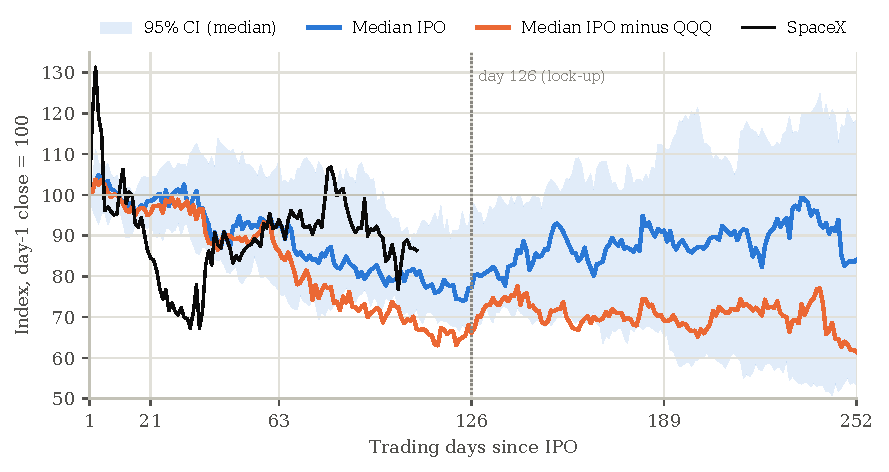
\includegraphics[width=\linewidth]{figures/v1/f1_path.pdf}
\caption{Median price path from the first close, 43 IPOs, with 95\% bootstrap band; median net of QQQ; SpaceX.}\label{fig:path}
\end{figure}
\begin{table*}[!htbp]\centering\small
\caption{Aftermarket returns by horizon}\label{tab:horizons}
\resizebox{\linewidth}{!}{
\begin{threeparttable}
\begin{tabular}{lrrrcrrc}
\toprule
Window & $n$ & Mean & Median & 95\% CI (median) & \% $<0$ & Med.\ vs QQQ & 95\% CI \\
\midrule
Offer to day-1 close (first-day return) & 43 & +37.1 & +19.2 & [+12, +32] & 16 & -- & -- \\
Day-1 close to day 5 & 43 & +5.3 & +4.2 & [$-$5, +7] & 42 & +3.7 & [$-$7, +5] \\
Day-1 close to day 21 & 43 & +2.5 & $-$1.5 & [$-$7, +5] & 53 & $-$4.5 & [$-$11, +4] \\
Day-1 close to day 63 & 43 & +2.7 & $-$7.0 & [$-$24, +8] & 58 & $-$13.8 & [$-$29, +1] \\
Day-1 close to day 126 & 42 & $-$11.7 & $-$22.7 & [$-$31, $-$2] & 64 & $-$33.8 & [$-$46, $-$15] \\
Day-1 close to day 252 & 41 & +0.2 & $-$15.9 & [$-$47, +18] & 56 & $-$38.6 & [$-$48, $-$10] \\
\bottomrule
\end{tabular}
\begin{tablenotes}[flushleft]\footnotesize
\item \textit{Notes:} Returns in percent. Horizons are trading days counted from the first close (day 1). ``vs QQQ'' subtracts the QQQ return over the same dates. Confidence intervals are 10,000-draw bootstrap percentile intervals of the median.
\end{tablenotes}
\end{threeparttable}
}
\end{table*}

\begin{table}[!htbp]\centering\small
\caption{Close-to-close returns, days 2 to 10}\label{tab:daily}

\begin{threeparttable}
\begin{tabular}{lrcrrrr}
\toprule
Day & Mean & 95\% CI & Median & \% up & $p$ ($t$-test) & Mean vs QQQ \\
\midrule
Day 2 & +1.63 & [$-$1.30, +4.78] & +0.95 & 58 & 0.31 & +1.57 \\
Day 3 & +2.63 & [$-$0.48, +5.94] & +3.75 & 67 & 0.12 & +2.23 \\
Day 4 & $-$0.94 & [$-$3.20, +1.56] & $-$2.68 & 28 & 0.45 & $-$0.80 \\
Day 5 & +1.40 & [$-$1.15, +4.64] & $-$0.20 & 47 & 0.35 & +1.11 \\
Day 6 & $-$2.57 & [$-$4.89, $-$0.39] & $-$1.42 & 35 & 0.032$^{**}$ & $-$2.23 \\
Day 7 & +0.81 & [$-$0.92, +2.69] & $-$0.17 & 47 & 0.39 & +0.76 \\
Day 8 & +0.62 & [$-$0.94, +2.19] & $-$0.07 & 49 & 0.45 & +0.54 \\
Day 9 & $-$0.11 & [$-$1.54, +1.35] & $-$0.47 & 44 & 0.88 & $-$0.38 \\
Day 10 & $-$0.45 & [$-$2.35, +1.80] & $-$0.44 & 44 & 0.68 & $-$0.16 \\
\bottomrule
\end{tabular}
\begin{tablenotes}[flushleft]\footnotesize
\item \textit{Notes:} Percent. 43 IPOs. Stars: $^{*}p<0.10$, $^{**}p<0.05$, $^{***}p<0.01$ (unadjusted). With nine days tested, the day-6 result does not survive a Bonferroni or Benjamini--Hochberg correction.
\end{tablenotes}
\end{threeparttable}

\end{table}


\subsection{Intraday: the opening print}
The median debut opens 23\% above its offer, closes 19\% above it and ends 7.5\% below its high; 60\% close below their open (Table~\ref{tab:intraday}). Debuts open late (median first hourly bar 12:30 ET, 14 IPOs since 2025). Volume concentrates in the first hour or two of trading, and the day's high came in the first trading hour for 10 of 14 hourly-data debuts (Table~\ref{tab:hourly}; Figure~\ref{fig:intraday}). Buying the open and holding to day 63 lost a median 11\%.

\begin{table*}[!htbp]\centering\small
\caption{Debut-day shape by size of the opening print}\label{tab:intraday}
\resizebox{\linewidth}{!}{
\begin{threeparttable}
\begin{tabular}{lrrrrrrrr}
\toprule
Opening print vs offer & $n$ & Open & Close & Open$\to$close & Close vs high & \% below open & Open$\to$D21 & Open$\to$D63 \\
\midrule
Open $<$10\% over offer & 12 & 0 & $-$2 & $-$0.8 & $-$4.3 & 58 & +2.4 & +9.7 \\
Open 10-40\% & 17 & +23 & +17 & $-$5.1 & $-$8.8 & 71 & $-$9.3 & $-$20.1 \\
Open $>$40\% & 14 & +80 & +79 & +1.4 & $-$11.3 & 50 & +0.4 & $-$17.2 \\
\midrule
All IPOs & 43 & +23 & +19 & $-$2.0 & $-$7.5 & 60 & $-$1.6 & $-$10.8 \\
\bottomrule
\end{tabular}
\begin{tablenotes}[flushleft]\footnotesize
\item \textit{Notes:} Medians in percent from daily open, high and close. The last two columns measure returns from the opening price, the entry available to a buyer without an allocation.
\end{tablenotes}
\end{threeparttable}
}
\end{table*}

\begin{table}[!htbp]\centering\small
\caption{Hourly profile of the first three sessions}\label{tab:hourly}

\begin{threeparttable}
\begin{tabular}{lrrrrrr}
\toprule
Bar (ET) & \multicolumn{3}{c}{Share of day's volume (\%)} & \multicolumn{3}{c}{Median bar return (\%)} \\ \cmidrule(lr){2-4}\cmidrule(lr){5-7} & Day 1 & Day 2 & Day 3 & Day 1 & Day 2 & Day 3 \\
\midrule
9:30 & -- & 35 & 37 & -- & $-$1.8 & +3.8 \\
10:30 & -- & 16 & 15 & -- & +1.1 & +0.6 \\
11:30 & 38 & 9 & 11 & $-$2.5 & $-$0.2 & $-$0.4 \\
12:30 & 40 & 8 & 8 & $-$2.2 & +0.5 & +0.2 \\
13:30 & 18 & 8 & 6 & $-$0.1 & +0.7 & $-$0.1 \\
14:30 & 16 & 7 & 10 & $-$2.6 & +0.1 & $-$0.1 \\
15:30 & 12 & 10 & 12 & $-$0.1 & $-$0.2 & $-$0.4 \\
\bottomrule
\end{tabular}
\begin{tablenotes}[flushleft]\footnotesize
\item \textit{Notes:} 14 IPOs since January 2025 whose hourly feed includes the debut session. Day-1 bars with fewer than four IPOs trading are omitted (most debuts open between 11:30 and 13:30 ET). The debut-day high fell in the first trading hour for 10 of 14 IPOs.
\end{tablenotes}
\end{threeparttable}

\end{table}

\begin{figure}[!htbp]\centering
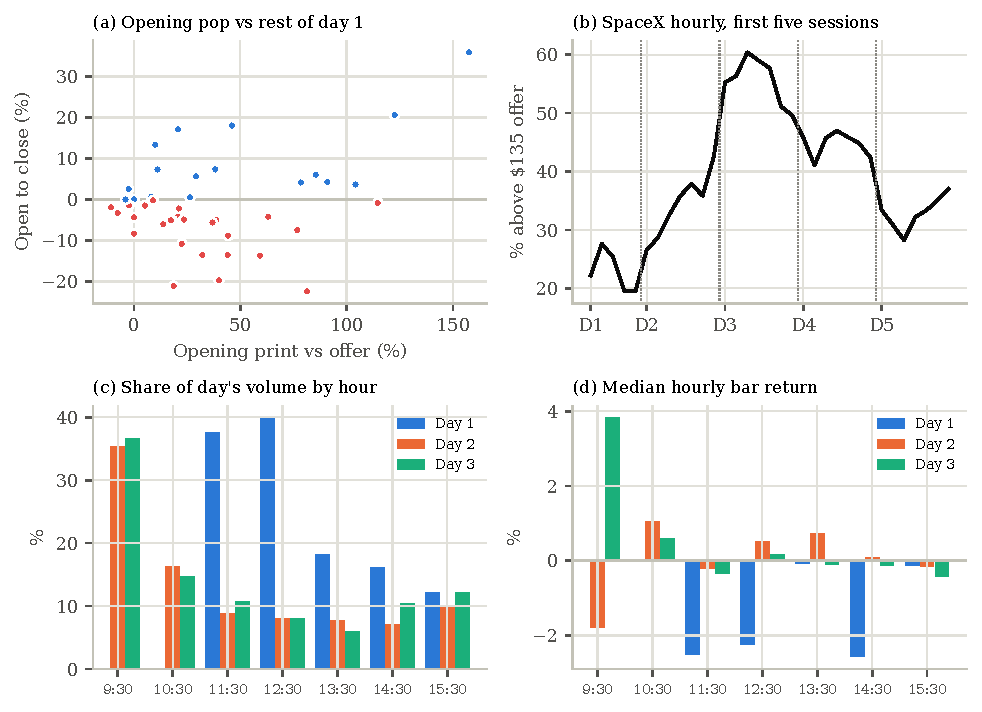
\includegraphics[width=\linewidth]{figures/v1/f4_intraday.pdf}
\caption{(a) Opening pop vs open-to-close. (b) SpaceX hourly, first five sessions. (c) Share of volume by hour. (d) Median hourly bar return.}\label{fig:intraday}
\end{figure}

\subsection{Market value, sector, season and rates}
The medians differ widely across buckets (Tables~\ref{tab:buckets} and~\ref{tab:regimes}; Figures~\ref{fig:sectors} and~\ref{fig:season}). Consumer internet faded first, fintech hardest and software, AI and semis least; Q4 and Q1 listings popped most; rising long yields went with weaker three-month returns. None of these differences survives correction (Kruskal--Wallis $q\geq0.57$). The market-level seasonal evidence is stronger: from 15 November of a midterm year the S\&P~500 rose over the next three months in 18 of 19 cases.

\begin{table}[!htbp]\centering\footnotesize
\caption{Median returns by market value, sector and listing quarter}\label{tab:buckets}

\begin{threeparttable}
\begin{tabular}{lrrrrcr}
\toprule
& $n$ & Pop & Day 21 & Day 63 & 95\% CI (day 63) & Day 126 \\
\midrule
\multicolumn{7}{l}{\textit{Panel A. Market value at offer}} \\
\quad Small $<$10B & 22 & +17 & +1 & $-$5 & [$-$22, +18] & $-$21 \\
\quad Mid 10-30B & 11 & +12 & $-$3 & $-$27 & [$-$35, +37] & $-$26 \\
\quad Large 30-100B & 9 & +41 & $-$4 & +2 & [$-$36, +30] & $-$24 \\
\quad Mega $\geq$100B & 1 & +19 & $-$15 & $-$6 & [--, --] & -- \\
\quad \footnotesize Kruskal--Wallis $p$ ($q$) & & \footnotesize 0.47 (0.88) & \footnotesize 0.79 (0.91) & \multicolumn{2}{c}{\footnotesize 0.79 (0.91)} & \footnotesize 0.79 (0.91) \\
\addlinespace
\multicolumn{7}{l}{\textit{Panel B. Sector}} \\
\quad Consumer \& leisure & 4 & +10 & +9 & 0 & [$-$34, +37] & +2 \\
\quad Consumer internet & 8 & +45 & $-$10 & $-$25 & [$-$35, +14] & $-$28 \\
\quad Fintech \& financials & 9 & +14 & +21 & $-$27 & [$-$35, +30] & $-$41 \\
\quad Healthcare & 4 & +13 & +4 & +27 & [+6, +49] & +11 \\
\quad Industrials, energy \& space & 6 & +23 & $-$4 & $-$15 & [$-$50, +3] & $-$26 \\
\quad Software, AI \& semis & 12 & +28 & $-$6 & $-$3 & [$-$14, +35] & $-$15 \\
\quad \footnotesize Kruskal--Wallis $p$ ($q$) & & \footnotesize 0.63 (0.91) & \footnotesize 0.10 (0.57) & \multicolumn{2}{c}{\footnotesize 0.21 (0.57)} & \footnotesize 0.18 (0.57) \\
\addlinespace
\multicolumn{7}{l}{\textit{Panel C. Listing quarter}} \\
\quad Q1 & 10 & +34 & $-$4 & $-$18 & [$-$30, +11] & $-$29 \\
\quad Q2 & 12 & +14 & +5 & $-$4 & [$-$26, +34] & +2 \\
\quad Q3 & 15 & +18 & $-$5 & $-$11 & [$-$28, +14] & $-$33 \\
\quad Q4 & 6 & +39 & +4 & $-$9 & [$-$30, +31] & $-$17 \\
\quad \footnotesize Kruskal--Wallis $p$ ($q$) & & \footnotesize 0.68 (0.91) & \footnotesize 0.43 (0.87) & \multicolumn{2}{c}{\footnotesize 0.82 (0.91)} & \footnotesize 0.33 (0.76) \\
\addlinespace
\bottomrule
\end{tabular}
\begin{tablenotes}[flushleft]\footnotesize
\item \textit{Notes:} Medians in percent. Pop is the first-day return from the offer; later columns are measured from the day-1 close. $q$ = Benjamini--Hochberg adjusted across all 28 bucket tests in Tables~\ref{tab:buckets} and \ref{tab:regimes}.
\end{tablenotes}
\end{threeparttable}

\end{table}

\begin{table}[!htbp]\centering\footnotesize
\caption{Median returns by macro regime and deal structure}\label{tab:regimes}

\begin{threeparttable}
\begin{tabular}{lrrrrcr}
\toprule
& $n$ & Pop & Day 21 & Day 63 & 95\% CI (day 63) & Day 126 \\
\midrule
\multicolumn{7}{l}{\textit{Panel A. 10-year yield, 3-month change before listing}} \\
\quad 10Y falling & 10 & +16 & $-$1 & $-$7 & [$-$30, +20] & $-$46 \\
\quad 10Y flat & 18 & +34 & +1 & +2 & [$-$28, +35] & $-$10 \\
\quad 10Y rising & 15 & +12 & $-$6 & $-$18 & [$-$27, +2] & $-$20 \\
\quad \footnotesize Kruskal--Wallis $p$ ($q$) & & \footnotesize 0.15 (0.57) & \footnotesize 0.69 (0.91) & \multicolumn{2}{c}{\footnotesize 0.41 (0.87)} & \footnotesize 0.20 (0.57) \\
\addlinespace
\multicolumn{7}{l}{\textit{Panel B. VIX level at listing}} \\
\quad VIX $<$16 & 17 & +14 & $-$6 & $-$11 & [$-$27, +14] & $-$6 \\
\quad VIX 16-22 & 19 & +19 & +5 & $-$2 & [$-$33, +14] & $-$27 \\
\quad VIX $>$22 & 7 & +56 & $-$4 & $-$23 & [$-$29, +43] & $-$36 \\
\quad \footnotesize Kruskal--Wallis $p$ ($q$) & & \footnotesize 0.15 (0.57) & \footnotesize 0.21 (0.57) & \multicolumn{2}{c}{\footnotesize 0.92 (0.97)} & \footnotesize 0.55 (0.91) \\
\addlinespace
\multicolumn{7}{l}{\textit{Panel C. Float (proceeds / market value)}} \\
\quad Float $<$8\% & 13 & +19 & $-$7 & $-$14 & [$-$35, +23] & $-$24 \\
\quad Float 8-15\% & 17 & +18 & $-$4 & $-$11 & [$-$28, +8] & $-$25 \\
\quad Float $>$15\% & 13 & +27 & +5 & +6 & [$-$27, +19] & $-$12 \\
\quad \footnotesize Kruskal--Wallis $p$ ($q$) & & \footnotesize 0.97 (0.97) & \footnotesize 0.22 (0.57) & \multicolumn{2}{c}{\footnotesize 0.77 (0.91)} & \footnotesize 0.63 (0.91) \\
\addlinespace
\multicolumn{7}{l}{\textit{Panel D. Final price vs first filed range}} \\
\quad At or below initial range & 14 & +4 & +1 & +14 & [$-$14, +30] & +7 \\
\quad Priced above initial range & 28 & +32 & $-$2 & $-$20 & [$-$28, $-$2] & $-$27 \\
\quad \footnotesize Kruskal--Wallis $p$ ($q$) & & \footnotesize 0.001 (0.040) & \footnotesize 0.94 (0.97) & \multicolumn{2}{c}{\footnotesize 0.11 (0.57)} & \footnotesize 0.037 (0.52) \\
\addlinespace
\bottomrule
\end{tabular}
\begin{tablenotes}[flushleft]\footnotesize
\item \textit{Notes:} As Table~\ref{tab:buckets}. 10Y rising/falling: more than $\pm$30bp over the three months before listing. Demand proxy: offer price relative to the first filed range \citep{hanley1993}; only 3 deals priced below range, so they are pooled with within-range deals.
\end{tablenotes}
\end{threeparttable}

\end{table}

\begin{figure}[!htbp]\centering
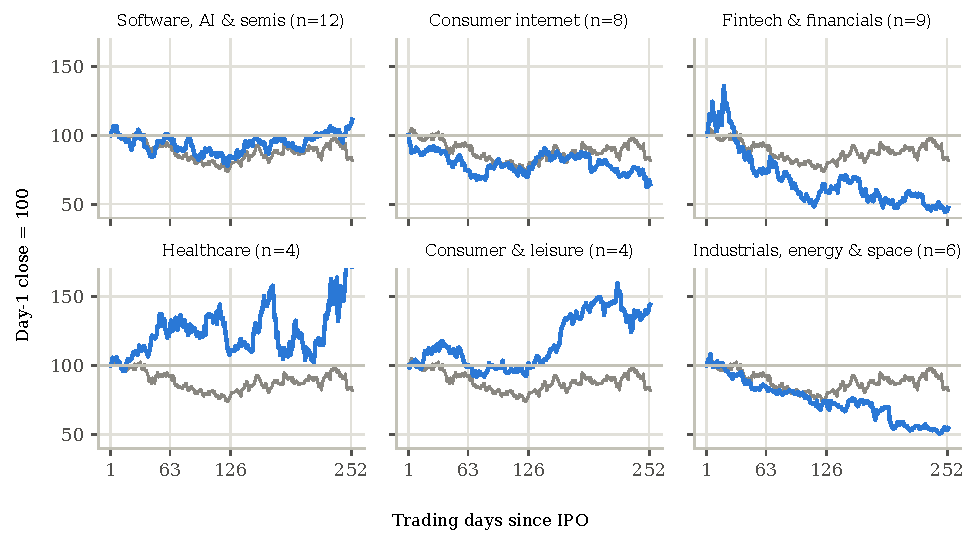
\includegraphics[width=\linewidth]{figures/v1/f2_sectors.pdf}
\caption{Median path from the first close by sector (blue) against all IPOs (grey).}\label{fig:sectors}
\end{figure}
\begin{figure}[!htbp]\centering
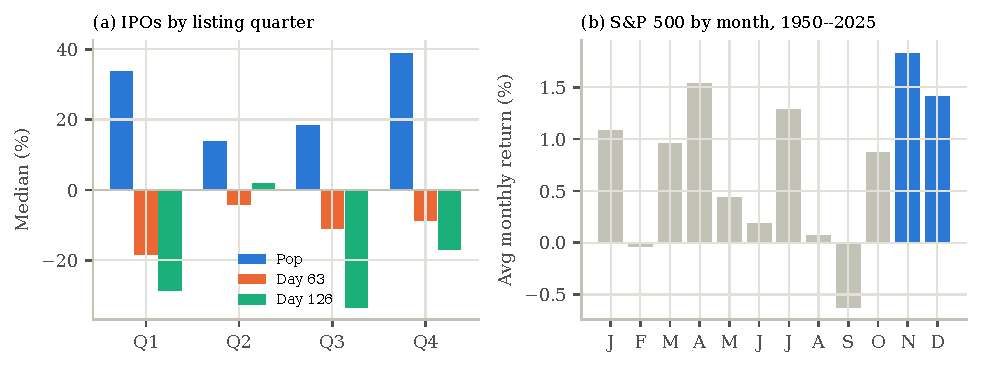
\includegraphics[width=\linewidth]{figures/v1/f8_season.pdf}
\caption{(a) IPO outcomes by listing quarter. (b) S\&P~500 average monthly return, 1950--2025.}\label{fig:season}
\end{figure}

\subsection{Demand and float}
Demand is the one deal characteristic that matters (Figure~\ref{fig:demand}; Table~\ref{tab:corr}). Deals priced above their first filed range popped 32\% against 4\%, and the price revision and the pop have a rank correlation of 0.67 ($q<0.001$), the partial-adjustment effect of \citet{hanley1993}. Those deals then gave back most ($-20\%$ at day 63, CI $-28\%$ to $-2\%$). Float, the fraction of shares sold, has no reliable relationship with any outcome.

\begin{figure}[!htbp]\centering
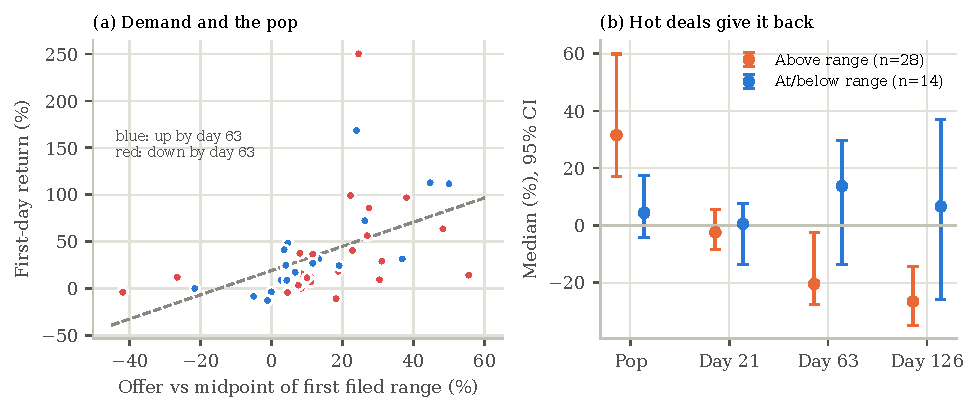
\includegraphics[width=\linewidth]{figures/v1/f3_demand.pdf}
\caption{(a) Price revision vs first-day return. (b) Medians with 95\% CIs by demand group.}\label{fig:demand}
\end{figure}
\begin{table}[!htbp]\centering\small
\caption{Spearman rank correlations}\label{tab:corr}

\begin{threeparttable}
\begin{tabular}{lrrrr}
\toprule
Pair & $n$ & $\rho$ & $p$ & $q$ (BH) \\
\midrule
Day-1 pop vs day-21 return & 43 & $+$0.04 & 0.80 & 0.88 \\
Day-1 pop vs day-63 return & 43 & $+$0.01 & 0.96 & 0.96 \\
Opening pop vs open-to-close & 43 & $+$0.07 & 0.66 & 0.80 \\
Market cap vs day-1 pop & 43 & $+$0.11 & 0.49 & 0.80 \\
10Y 3-month change vs day-63 return & 43 & $-$0.14 & 0.37 & 0.80 \\
VIX vs day-1 pop & 43 & $+$0.23 & 0.13 & 0.74 \\
Day 1-5 squeeze vs day 5-63 return (non-overlapping) & 43 & $+$0.09 & 0.57 & 0.80 \\
Float \% vs day-1 pop & 43 & $-$0.08 & 0.61 & 0.80 \\
Float \% vs day-63 return & 43 & $+$0.13 & 0.42 & 0.80 \\
Price revision vs day-1 pop & 42 & $+$0.67 & $<$0.001 & $<$0.001 \\
Price revision vs day-63 return & 42 & $-$0.15 & 0.35 & 0.80 \\
\bottomrule
\end{tabular}
\begin{tablenotes}[flushleft]\footnotesize
\item \textit{Notes:} Returns measured from the day-1 close unless stated. The squeeze test uses non-overlapping windows (days 1--5 vs days 5--63). $q$ adjusts across the 11 correlations.
\end{tablenotes}
\end{threeparttable}

\end{table}


% ===========================================================================
\section{Positioning and crowding: what sets the size of the fade}

\subsection{The market state at listing}
Figure~\ref{fig:psi} plots PSI with the large listings marked; Appendix Table~\ref{tab:states} gives each listing's state. Fifteen of 22 large listings came with PSI above its median, consistent with issuers timing deals into strong markets \citep{lowry2002}.

\begin{figure}[!htbp]\centering
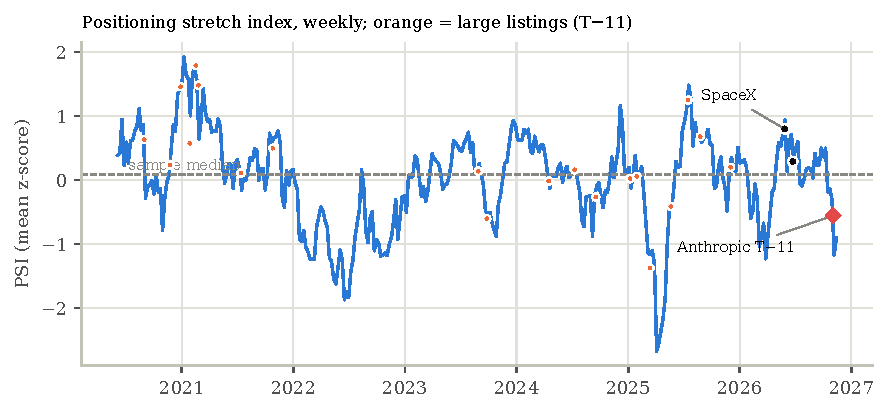
\includegraphics[width=\linewidth]{figures/v2/f1_psi.pdf}
\caption{Positioning stretch index (weekly) and its value 11 sessions before each large listing.}\label{fig:psi}
\end{figure}

\subsection{Positioning and the IPO stock}
IPOs that list into a stretched market pop more and fade much harder (Tables~\ref{tab:terciles}--\ref{tab:robust}; Figure~\ref{fig:ipo}). PSI at listing and the day-63 return have a rank correlation of $-0.51$ ($q=0.006$; $-0.44$ net of QQQ). The strongest ingredient is the high-beta spread ($\rho=-0.52$). Controlling for demand and size, positioning explains the fade and demand explains the pop. A hot book alone does not produce a deep fade: above-range deals in stretched markets went $+35\%$ then $-28\%$, while above-range deals in other markets went $+32\%$ then $-5\%$. The result holds without 2021 and leaving out each year in turn. A year-block bootstrap interval ($-0.59$ to $+0.03$) just includes zero, a reminder that stretched listings cluster in time.

\begin{table}[!htbp]\centering\small
\caption{IPO outcomes by positioning at listing (PSI terciles)}\label{tab:terciles}

\begin{threeparttable}
\begin{tabular}{lrrrrrr}
\toprule
PSI tercile & $n$ & Median PSI & Pop & Day 21 & Day 63 & Day 63 vs QQQ \\
\midrule
Low PSI & 15 & $-$0.11 & +9 & +5 & +19 & +8 \\
Mid PSI & 14 & 0.16 & +29 & $-$2 & +4 & $-$3 \\
High PSI & 14 & 0.78 & +27 & $-$4 & $-$28 & $-$33 \\
\bottomrule
\end{tabular}
\begin{tablenotes}[flushleft]\footnotesize
\item \textit{Notes:} Medians in percent. PSI is the last weekly reading before listing. Returns after day 1 are measured from the first close.
\end{tablenotes}
\end{threeparttable}

\end{table}

\begin{figure}[!htbp]\centering
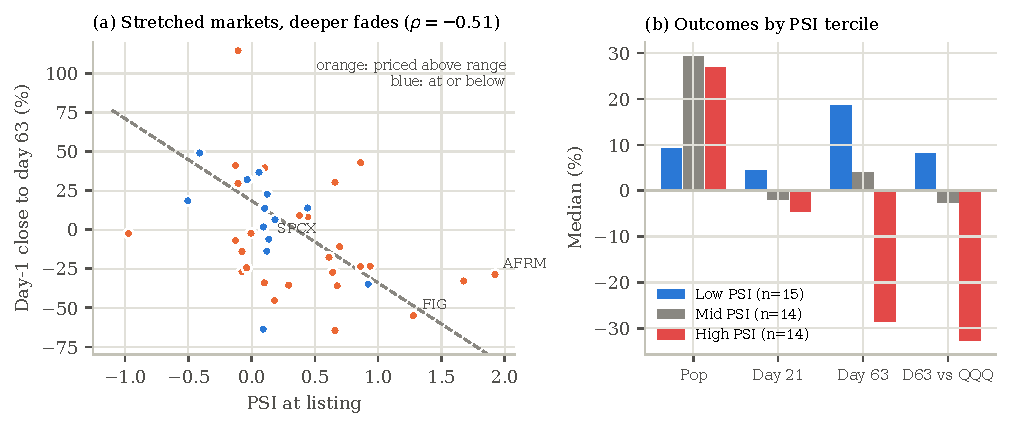
\includegraphics[width=\linewidth]{figures/v2/f3_ipo.pdf}
\caption{(a) PSI at listing vs the return from the first close to day 63. (b) Outcomes by PSI tercile.}\label{fig:ipo}
\end{figure}
\begin{table}[!htbp]\centering\footnotesize
\caption{Positioning at listing and IPO outcomes: rank correlations}\label{tab:ipocorr}

\begin{threeparttable}
\begin{tabular}{llrrr}
\toprule
State variable & Outcome & $\rho$ & $p$ & $q$ \\
\midrule
High beta vs low vol (SPHB/SPLV), 63d & Day 63 & $-$0.51 & $<$0.001 & 0.006 \\
Positioning stretch index (PSI) & Day 63 & $-$0.51 & $<$0.001 & 0.006 \\
High beta vs low vol (SPHB/SPLV), 63d & Day 63 vs QQQ & $-$0.48 & 0.001 & 0.009 \\
Positioning stretch index (PSI) & Day 63 vs QQQ & $-$0.44 & 0.003 & 0.018 \\
S\&P 500 return, 63d & Pop & 0.43 & 0.004 & 0.020 \\
Bitcoin return, 63d & Day 63 & $-$0.38 & 0.013 & 0.043 \\
Bitcoin return, 63d & Day 63 vs QQQ & $-$0.38 & 0.013 & 0.043 \\
Positioning stretch index (PSI) & Pop & 0.37 & 0.015 & 0.045 \\
Bitcoin return, 63d & Pop & 0.36 & 0.017 & 0.045 \\
High beta vs low vol (SPHB/SPLV), 63d & Pop & 0.34 & 0.026 & 0.063 \\
VIX / VIX3M & Pop & $-$0.30 & 0.054 & 0.117 \\
S\&P 500 realised vol, 21d & Day 63 & 0.28 & 0.069 & 0.137 \\
S\&P 500 return, 63d & Day 63 & $-$0.25 & 0.10 & 0.189 \\
S\&P 500 realised vol, 21d & Day 63 vs QQQ & 0.24 & 0.12 & 0.198 \\
\bottomrule
\end{tabular}
\begin{tablenotes}[flushleft]\footnotesize
\item \textit{Notes:} 43 IPOs. The 14 smallest $p$-values of 24 tests (8 state variables $\times$ 3 outcomes); $q$ adjusts across all 24.
\end{tablenotes}
\end{threeparttable}

\end{table}

\begin{table}[!htbp]\centering\footnotesize
\caption{Cross-sectional regressions: positioning versus demand}\label{tab:iporeg}

\begin{threeparttable}
\begin{tabular}{llrrrrr}
\toprule
Dependent variable & Spec. & PSI & Price revision & log market value & $R^2$ & $n$ \\
\midrule
First-day return & (1) & 0.36 (2.3) & -- & -- & 0.17 & 42 \\
 & (2) & 0.21 (1.3) & 1.01 (2.7) & 0.06 (1.0) & 0.30 & 42 \\
Day 63 return & (1) & $-$0.53 ($-$1.8) & -- & -- & 0.28 & 42 \\
 & (2) & $-$0.56 ($-$2.0) & 0.17 (0.3) & 0.06 (0.6) & 0.29 & 42 \\
Day 63 vs QQQ & (1) & $-$0.50 ($-$1.8) & -- & -- & 0.27 & 42 \\
 & (2) & $-$0.52 ($-$2.0) & 0.08 (0.1) & 0.07 (0.8) & 0.28 & 42 \\
\bottomrule
\end{tabular}
\begin{tablenotes}[flushleft]\footnotesize
\item \textit{Notes:} OLS with HC3 robust $t$-statistics in brackets. Returns as decimals. Price revision = offer vs midpoint of the first filed range. Demand drives the pop; positioning drives the fade.
\end{tablenotes}
\end{threeparttable}

\end{table}

\begin{table}[!htbp]\centering\footnotesize
\caption{Positioning and demand together}\label{tab:2x2}

\begin{threeparttable}
\begin{tabular}{lrrrrrr}
\toprule
& \multicolumn{3}{c}{Priced above first range} & \multicolumn{3}{c}{At or below range} \\ \cmidrule(lr){2-4}\cmidrule(lr){5-7} PSI at listing & $n$ & Pop & Day 63 & $n$ & Pop & Day 63 \\
\midrule
High PSI & 12 & +35 & $-$28 & 2 & +3 & $-$35 \\
Low or mid PSI & 16 & +32 & $-$5 & 12 & +4 & +16 \\
\bottomrule
\end{tabular}
\begin{tablenotes}[flushleft]\footnotesize
\item \textit{Notes:} Medians in percent. Day 63 measured from the first close.
\end{tablenotes}
\end{threeparttable}

\end{table}

\begin{table}[!htbp]\centering\footnotesize
\caption{Robustness of the PSI--fade relationship}\label{tab:robust}

\begin{threeparttable}
\begin{tabular}{lrrr}
\toprule
Test & $n$ & $\rho$ & $p$ \\
\midrule
Full sample, day 63 & 43 & $-$0.51 & $<$0.001 \\
Full sample, day 63 vs QQQ & 43 & $-$0.44 & 0.003 \\
Excluding 2021 listings, day 63 & 34 & $-$0.41 & 0.015 \\
Excluding 2021 listings, day 63 vs QQQ & 34 & $-$0.37 & 0.031 \\
Leave one listing year out, day 63 (range) & -- & $-$0.41 to $-$0.55 & -- \\
Year-block bootstrap 95\% CI, day 63 & -- & [$-$0.59, 0.03] & -- \\
Full sample, first-day return & 43 & 0.37 & 0.015 \\
PSI vs price revision & 42 & 0.35 & 0.021 \\
\bottomrule
\end{tabular}
\begin{tablenotes}[flushleft]\footnotesize
\item \textit{Notes:} Spearman correlations between PSI at listing and the outcome. The year-block bootstrap resamples listing years with replacement (5,000 draws), allowing for clustering of IPOs in hot windows.
\end{tablenotes}
\end{threeparttable}

\end{table}


\subsection{Crowded trades, within buckets}
The signal comes from crowded trades around the IPO rather than from frenzied trading in the stock (Table~\ref{tab:crowdcorr}). The crowding composite predicts a bigger pop ($\rho=0.44$, $q=0.03$) and a deeper fade ($\rho=-0.37$). Crowding into new issues and into the IPO's own sector mainly inflates the pop; crowded high beta and Bitcoin mainly predict the fade; momentum crowding alone has no signal. Turnover in the IPO itself is unrelated to what follows.

The crowding signal survives the earlier bucketings (Table~\ref{tab:crowdbuckets}; Figure~\ref{fig:crowdbuckets}). Crowded listings had lower day-63 medians in every market-value, rate, float and demand bucket and in most quarters, VIX regimes and sectors. A permutation that shuffles crowding only within buckets gives $p$ between 0.010 and 0.028 for market value, quarter, rates, VIX, float and demand; sector is marginal (0.074). Crowding and PSI largely overlap (Table~\ref{tab:crowdrace}).

\begin{table}[!htbp]\centering\footnotesize
\caption{Crowded trades at listing and IPO outcomes: rank correlations}\label{tab:crowdcorr}

\begin{threeparttable}
\begin{tabular}{lrrrrr}
\toprule
Crowding signal & Pop & Day 21 & Day 63 & D63 vs QQQ & Day 5$\to$63 \\
\midrule
High beta vs low vol, 63d & 0.28 & $-$0.21 & $-$0.44$^{\dagger}$ & $-$0.41$^{\dagger}$ & $-$0.34$^{*}$ \\
Momentum vs market, 63d & 0.11 & $-$0.01 & 0.08 & 0.06 & 0.00 \\
Bitcoin, 63d & 0.31 & $-$0.14 & $-$0.34$^{*}$ & $-$0.34$^{*}$ & $-$0.28 \\
Recent IPOs (IPO ETF) vs S\&P, 63d & 0.42$^{\dagger}$ & $-$0.07 & $-$0.18 & $-$0.17 & $-$0.10 \\
Own sector ETF vs S\&P, 63d & 0.43$^{\dagger}$ & $-$0.23 & $-$0.28 & $-$0.27 & $-$0.21 \\
Crowding composite & 0.44$^{\dagger}$ & $-$0.24 & $-$0.37$^{*}$ & $-$0.37$^{*}$ & $-$0.32 \\
\midrule
Day-1 turnover (vol / shares sold) & -- & $-$0.14 & 0.05 & 0.06 & 0.03 \\
Days 1--5 turnover & -- & $-$0.03 & 0.04 & 0.06 & $-$0.04 \\
\bottomrule
\end{tabular}
\begin{tablenotes}[flushleft]\footnotesize
\item \textit{Notes:} Spearman $\rho$ across 43 IPOs. $^{\dagger}q<0.05$, $^{*}q<0.10$ (Benjamini--Hochberg across all 64 signal--outcome tests). Market crowding measured at the last close before listing; turnover is observed on and after day 1, so it is not related to the pop. Sector ETFs: IGV, FDN, ARKF, XLV, XLY, XLI.
\end{tablenotes}
\end{threeparttable}

\end{table}

\begin{table}[!htbp]\centering\scriptsize
\caption{Crowded versus not crowded within each bucket}\label{tab:crowdbuckets}

\begin{threeparttable}
\begin{tabular}{lrrrrrrc}
\toprule
Bucket & $n$ cr./not & Pop cr. & Pop not & D63 cr. & D63 not & $\rho$ (D63) & Cr.\ worse \\
\midrule
\multicolumn{8}{l}{\textit{Market cap}: perm.\ $p=0.017$; FE $t$ (pop) $=3.1$, FE $t$ (D63) $=$-$1.7$; crowded worse in 3 of 3} \\
\quad Large \& mega (\$30B+) & 6 / 4 & +63 & +27 & $-$15 & +4 & $-$0.09 & yes \\
\quad Mid 10-30B & 6 / 5 & +34 & +9 & $-$28 & $-$2 & $-$0.54 & yes \\
\quad Small $<$10B & 10 / 12 & +21 & +14 & $-$19 & +3 & $-$0.42 & yes \\
\addlinespace
\multicolumn{8}{l}{\textit{Sector}: perm.\ $p=0.074$; FE $t$ (pop) $=3.0$, FE $t$ (D63) $=$-$1.4$; crowded worse in 3 of 5} \\
\quad Consumer \& leisure & 1 / 3 & +11 & +9 & $-$34 & +19 & -- & yes \\
\quad Consumer internet & 6 / 2 & +56 & +12 & $-$23 & $-$31 & 0.36 & no \\
\quad Fintech \& financials & 7 / 2 & +24 & $-$4 & $-$28 & +6 & $-$0.33 & yes \\
\quad Healthcare & 0 / 4 & -- & +13 & -- & +27 & -- & -- \\
\quad Industrials, energy \& space & 2 / 4 & +8 & +28 & $-$35 & $-$13 & $-$0.60 & yes \\
\quad Software, AI \& semis & 6 / 6 & +52 & +20 & $-$1 & $-$3 & $-$0.29 & no \\
\addlinespace
\multicolumn{8}{l}{\textit{Listing quarter}: perm.\ $p=0.016$; FE $t$ (pop) $=3.1$, FE $t$ (D63) $=$-$1.5$; crowded worse in 3 of 4} \\
\quad Q1 & 8 / 2 & +45 & +13 & $-$25 & +155 & $-$0.65 & yes \\
\quad Q2 & 4 / 8 & +28 & +10 & $-$20 & +10 & $-$0.34 & yes \\
\quad Q3 & 8 / 7 & +21 & +12 & $-$20 & $-$2 & $-$0.33 & yes \\
\quad Q4 & 2 / 4 & +99 & +33 & +10 & $-$9 & $-$0.14 & no \\
\addlinespace
\multicolumn{8}{l}{\textit{10Y trend}: perm.\ $p=0.015$; FE $t$ (pop) $=2.7$, FE $t$ (D63) $=$-$1.9$; crowded worse in 3 of 3} \\
\quad 10Y falling & 5 / 5 & +14 & +27 & $-$28 & +9 & $-$0.52 & yes \\
\quad 10Y flat & 10 / 8 & +75 & +13 & $-$10 & +15 & $-$0.38 & yes \\
\quad 10Y rising & 7 / 8 & +41 & +12 & $-$27 & $-$10 & $-$0.28 & yes \\
\addlinespace
\multicolumn{8}{l}{\textit{VIX at listing}: perm.\ $p=0.010$; FE $t$ (pop) $=2.7$, FE $t$ (D63) $=$-$2.1$; crowded worse in 2 of 3} \\
\quad VIX 16-22 & 7 / 12 & +37 & +15 & $-$33 & +8 & $-$0.62 & yes \\
\quad VIX $<$16 & 9 / 8 & +18 & +11 & $-$14 & $-$3 & $-$0.34 & yes \\
\quad VIX $>$22 & 6 / 1 & +69 & +56 & +3 & $-$45 & $-$0.11 & no \\
\addlinespace
\multicolumn{8}{l}{\textit{Float}: perm.\ $p=0.018$; FE $t$ (pop) $=2.9$, FE $t$ (D63) $=$-$1.8$; crowded worse in 3 of 3} \\
\quad Float 8-15\% & 10 / 7 & +21 & +16 & $-$19 & $-$2 & $-$0.39 & yes \\
\quad Float $<$8\% & 7 / 6 & +37 & +9 & $-$23 & 0 & $-$0.36 & yes \\
\quad Float $>$15\% & 5 / 8 & +48 & +22 & $-$27 & +8 & $-$0.40 & yes \\
\addlinespace
\multicolumn{8}{l}{\textit{Pricing vs range}: perm.\ $p=0.028$; FE $t$ (pop) $=2.5$, FE $t$ (D63) $=$-$2.0$; crowded worse in 2 of 2} \\
\quad Above range & 17 / 11 & +41 & +27 & $-$24 & $-$14 & $-$0.25 & yes \\
\quad At or below range & 4 / 10 & $-$4 & +9 & $-$25 & +21 & $-$0.55 & yes \\
\addlinespace
\multicolumn{8}{l}{\textit{PSI tercile}: perm.\ $p=0.204$; FE $t$ (pop) $=2.3$, FE $t$ (D63) $=$-$1.1$; crowded worse in 1 of 3} \\
\quad High PSI & 12 / 2 & +33 & +21 & $-$28 & $-$35 & 0.26 & no \\
\quad Low PSI & 4 / 11 & +72 & +9 & +35 & $-$2 & $-$0.12 & no \\
\quad Mid PSI & 6 / 8 & +28 & +29 & $-$10 & +8 & $-$0.53 & yes \\
\addlinespace
\bottomrule
\end{tabular}
\begin{tablenotes}[flushleft]\footnotesize
\item \textit{Notes:} Crowded = crowding composite above its cohort median. Medians in percent; D63 from the first close. perm.\ $p$: two-sided test that shuffles the composite only within buckets (5,000 draws). FE $t$: HC3 $t$-statistic on the composite in OLS with bucket fixed effects.
\end{tablenotes}
\end{threeparttable}

\end{table}

\begin{figure}[!htbp]\centering
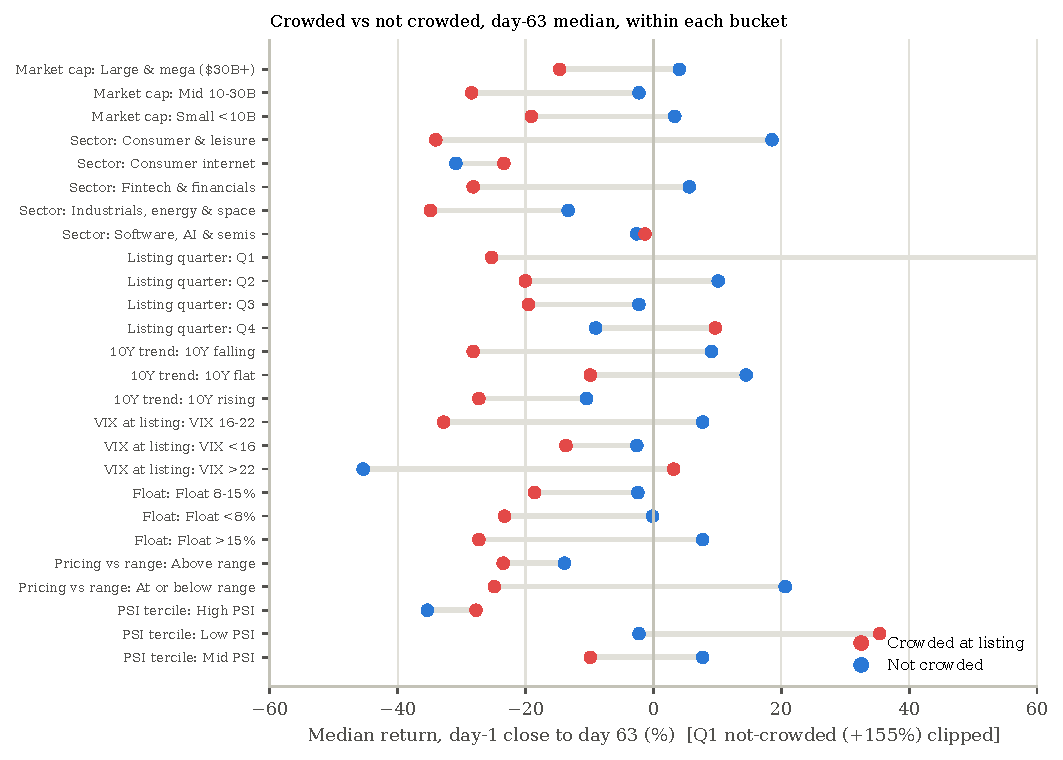
\includegraphics[width=0.95\linewidth]{figures/v2/f6_crowd_buckets.pdf}
\caption{Median day-63 return for crowded (red) and not-crowded (blue) listings within each bucket.}\label{fig:crowdbuckets}
\end{figure}
\begin{table}[!htbp]\centering\footnotesize
\caption{Crowding, demand and positioning together}\label{tab:crowdrace}

\begin{threeparttable}
\begin{tabular}{lrrrrr}
\toprule
Outcome & Crowding alone & Crowding & Price revision & Crowding & PSI \\ & (1) & \multicolumn{2}{c}{(2)} & \multicolumn{2}{c}{(3)} \\
\midrule
Pop & 0.32 (3.2) & 0.19 (1.8) & 0.96 (2.7) & 0.17 (0.9) & 0.23 (0.9) \\
Day 63 & $-$0.30 ($-$1.9) & $-$0.31 ($-$2.4) & 0.00 (0.0) & 0.05 (0.4) & $-$0.56 ($-$1.7) \\
D63 vs QQQ & $-$0.29 ($-$1.9) & $-$0.30 ($-$2.5) & $-$0.07 ($-$0.1) & 0.03 (0.3) & $-$0.52 ($-$1.6) \\
\bottomrule
\end{tabular}
\begin{tablenotes}[flushleft]\footnotesize
\item \textit{Notes:} OLS coefficients with HC3 $t$-statistics in brackets; 42--43 IPOs. The crowding composite and PSI share two components (high beta vs low vol and Bitcoin), so model (3) mainly asks which summary fits better.
\end{tablenotes}
\end{threeparttable}

\end{table}


% ===========================================================================
\section{Cross-asset effects and liquidity transfer}

\subsection{The average large listing}
Across 11 large listings, the ten sessions before listing look ordinary for every asset (Table~\ref{tab:xasset}; Figure~\ref{fig:xasset}). Bitcoin rose 3.6\% on average ($p=0.67$). The week after listing is softer (S\&P~500 $-1.2\%$, VIX $+2.6$ points), followed by a rebound. None of this survives correction for 56 tests, and the averages lean on CoreWeave, which listed days before the April 2025 tariff sell-off. In the hour a large IPO opens, QQQ, SPY and small caps fell in all four large recent cases (Table~\ref{tab:hour}); that is four observations.

\begin{table}[!htbp]\centering\footnotesize
\caption{Cross-asset moves around 11 large US listings}\label{tab:xasset}

\begin{threeparttable}
\begin{tabular}{lrrrrrr}
\toprule
Asset & T$-$10 to T$-$1 & Listing day & T+1 to T+5 & T+6 to T+20 & Median T+1--5 & min $q$ \\
\midrule
S\&P 500 (SPY) & +0.2 & $-$0.2 & $-$1.2$^{**}$ & +3.1$^{**}$ & +0.3 & 0.48 \\
Nasdaq 100 (QQQ) & $-$0.5 & $-$0.6 & $-$1.1$^{*}$ & +3.8$^{*}$ & +0.3 & 0.48 \\
Small caps (IWM) & +1.9 & +0.1 & $-$1.8$^{**}$ & +1.9 & $-$0.7 & 0.48 \\
Speculative growth (ARKK) & +0.7 & $-$0.5 & $-$2.8$^{*}$ & +4.2 & $-$4.0 & 0.48 \\
Semis (SMH) & $-$1.1 & $-$0.6 & $-$1.2 & +5.9 & $-$1.2 & 0.48 \\
Software (IGV) & +0.3 & $-$0.7 & $-$1.2 & +4.2$^{*}$ & $-$0.7 & 0.48 \\
Bitcoin & +3.6 & +0.1 & +0.4 & +10.5 & +0.1 & 0.48 \\
Gold (GLD) & $-$0.1 & 0.0 & $-$0.1 & +1.1 & +0.5 & 0.83 \\
Long Treasuries (TLT) & $-$0.3 & $-$0.2 & +0.2 & $-$1.0 & +0.4 & 0.83 \\
Dollar (UUP) & +0.2 & +0.1 & +0.2 & $-$0.3 & +0.1 & 0.61 \\
High yield (HYG) & +0.2 & 0.0 & $-$0.5$^{**}$ & +0.9 & $-$0.2 & 0.48 \\
VIX (points) & +0.1 & +0.3 & +2.6$^{**}$ & $-$2.4 & +0.1 & 0.48 \\
US 10Y (bp) & +3.0 & +1.2 & $-$2.0 & +7.4 & $-$1.5 & 0.77 \\
Recent IPOs (IPO ETF) & +1.3 & $-$0.5 & $-$1.6 & +2.7 & +0.9 & 0.61 \\
\bottomrule
\end{tabular}
\begin{tablenotes}[flushleft]\footnotesize
\item \textit{Notes:} Average across events; percent except VIX (points) and US 10Y (basis points). Stars from a permutation test against 10,000 draws of 11 random dates since mid-2020 ($^{*}p<0.10$, $^{**}p<0.05$). min $q$ is the smallest Benjamini--Hochberg $q$ across the asset's four windows (56 tests in total); none is below 0.30.
\end{tablenotes}
\end{threeparttable}

\end{table}

\begin{figure}[!htbp]\centering
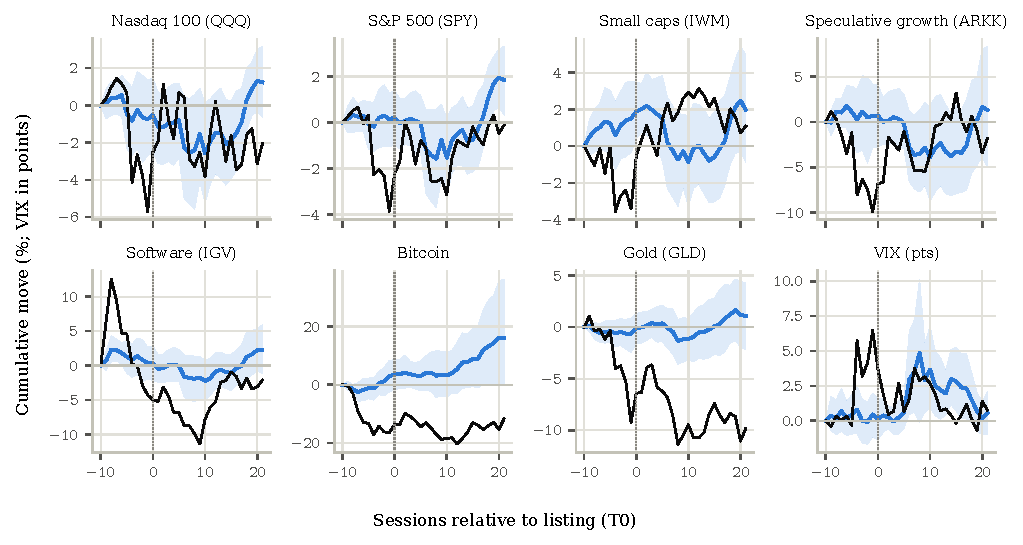
\includegraphics[width=\linewidth]{figures/v1/f6_xasset.pdf}
\caption{Average cumulative move around 11 large listings (blue, 90\% band) and SpaceX (black).}\label{fig:xasset}
\end{figure}
\begin{table}[!htbp]\centering\small
\caption{Abnormal return of other assets in the hour an IPO opens}\label{tab:hour}

\begin{threeparttable}
\begin{tabular}{lrrrrrr}
\toprule
Asset & \multicolumn{3}{c}{Large deals ($n=4$)} & \multicolumn{2}{c}{All ($n=14$)} & SpaceX \\ \cmidrule(lr){2-4}\cmidrule(lr){5-6} & bp & \% down & $t$ & bp & \% down & bp \\
\midrule
QQQ & $-$22 & 100\% & $-$2.8 & $-$6 & 71\% & $-$41 \\
SPY & $-$23 & 100\% & $-$2.2 & $-$5 & 57\% & $-$42 \\
Bitcoin & $-$21 & 75\% & $-$1.2 & $-$6 & 50\% & $-$50 \\
Gold (GLD) & $-$3 & 50\% & $-$0.0 & $-$1 & 50\% & $-$18 \\
ARKK & $-$51 & 75\% & $-$2.3 & $-$19 & 64\% & $-$82 \\
IWM & $-$32 & 100\% & $-$3.2 & $+$3 & 36\% & $-$51 \\
\bottomrule
\end{tabular}
\begin{tablenotes}[flushleft]\footnotesize
\item \textit{Notes:} Return in the IPO's first trading hour minus the average of the same clock hour over the prior 20 sessions, in basis points. Large deals: proceeds of \$1.4bn or more (CoreWeave, Medline, SpaceX, Venture Global).
\end{tablenotes}
\end{threeparttable}

\end{table}


\subsection{Conditioning on positioning}
If mega-IPOs drained liquidity only in stretched markets, the event$\times$PSI interaction would be negative. The state-matched placebo (Table~\ref{tab:split}) and the panel regressions (Table~\ref{tab:reg}; Figure~\ref{fig:inter}) say otherwise. In stretched markets risk assets tend to \emph{rise} into large listings. The only interaction that survives correction is positive: the high-beta spread gains an extra 2.5\% per unit of PSI ($q=0.05$). Negative interactions for the Nasdaq and gold ($q=0.12$--$0.15$) and several single-variable correlations (Table~\ref{tab:varcorr}) are consistent with a ``sell what you can'' response but do not survive correction.

\begin{table}[!htbp]\centering\footnotesize
\caption{Event windows split by positioning, against a state-matched placebo}\label{tab:split}
\resizebox{\linewidth}{!}{
\begin{threeparttable}
\begin{tabular}{lrrrrrrrr}
\toprule
& \multicolumn{4}{c}{T$-$10 to T$-$1} & \multicolumn{4}{c}{Listing day to T+5} \\ \cmidrule(lr){2-5}\cmidrule(lr){6-9} Asset & Stretched & Placebo & Not str. & Placebo & Stretched & Placebo & Not str. & Placebo \\
\midrule
S\&P 500 & +0.41 & +0.58 & +1.48 & +0.68 & $-$0.08 & +0.32 & $-$1.23 & +0.44 \\
Nasdaq 100 & $-$0.44 & +0.59 & +1.94 & +0.91 & $-$0.30 & +0.29 & $-$1.42 & +0.58 \\
Small caps & +2.09$^{*}$ & +0.36 & +0.84 & +0.58 & $-$0.32 & +0.13 & $-$1.80$^{*}$ & +0.44 \\
Spec. growth (ARKK) & +0.30 & $-$0.15 & +2.85 & +0.64 & $-$1.59 & $-$0.40 & $-$2.86 & +0.53 \\
Bitcoin & +5.74 & +1.12 & +0.96 & +1.40 & +2.57 & +0.05 & $-$0.32 & +1.52 \\
Gold & $-$0.20 & +0.59 & +1.54 & +0.47 & +0.13 & +0.32 & +0.88 & +0.36 \\
High beta - low vol & +2.16$^{*}$ & +0.14 & +0.89 & +0.94 & $-$0.70 & +0.06 & $-$2.29$^{*}$ & +0.53 \\
Momentum - market & $-$0.83 & $-$0.12 & +1.23 & +0.12 & $-$0.07 & $-$0.13 & $-$0.59 & +0.05 \\
Cross-asset momentum L/S & +1.11 & +1.46 & $-$3.80 & $-$0.51 & $-$0.25 & +0.53 & $-$0.32 & 0.00 \\
\bottomrule
\end{tabular}
\begin{tablenotes}[flushleft]\footnotesize
\item \textit{Notes:} Average log return in percent. Stretched = PSI at T$-$11 above its sample median (15 of 22 events). Placebo = average over all days in the same PSI half. Stars: permutation $p$ of the event average against 5,000 draws from the matched placebo days ($^{*}p<0.10$, $^{**}p<0.05$).
\end{tablenotes}
\end{threeparttable}
}
\end{table}

\begin{table}[!htbp]\centering\scriptsize
\caption{Panel regressions: does a large listing in a stretched market move assets more than a stretched day?}\label{tab:reg}
\resizebox{\linewidth}{!}{
\begin{threeparttable}
\begin{tabular}{llrrrrr}
\toprule
Asset & Window & PSI ($t$) & Event ($t$) & Event$\times$PSI ($t$) & $p$ & $q$ \\
\midrule
S\&P 500 & pre & $-$0.24 ($-$0.8) & 0.41 (0.9) & $-$0.55 ($-$1.2) & 0.23 & 0.49 \\
S\&P 500 & post & $-$0.10 ($-$0.5) & $-$1.50 ($-$1.7) & 1.99 (1.6) & 0.11 & 0.35 \\
S\&P 500 & late & $-$0.12 ($-$0.3) & 1.09 (1.2) & $-$0.07 ($-$0.1) & 0.95 & 0.95 \\
Nasdaq 100 & pre & $-$0.31 ($-$0.8) & 0.26 (0.4) & $-$1.65 ($-$2.3) & 0.022 & 0.15 \\
Nasdaq 100 & post & $-$0.23 ($-$0.9) & $-$1.83 ($-$1.7) & 2.34 (1.5) & 0.13 & 0.35 \\
Nasdaq 100 & late & $-$0.45 ($-$0.8) & 1.27 (1.1) & $-$0.11 ($-$0.1) & 0.94 & 0.95 \\
Small caps & pre & $-$0.46 ($-$1.3) & 1.30 (2.1) & 0.31 (0.4) & 0.71 & 0.91 \\
Small caps & post & $-$0.15 ($-$0.6) & $-$1.83 ($-$1.9) & 2.30 (1.8) & 0.069 & 0.35 \\
Small caps & late & $-$0.34 ($-$0.7) & 0.65 (0.6) & 0.30 (0.2) & 0.83 & 0.94 \\
Spec. growth (ARKK) & pre & $-$0.83 ($-$1.1) & 2.45 (2.4) & $-$3.56 ($-$1.6) & 0.11 & 0.35 \\
Spec. growth (ARKK) & post & $-$0.58 ($-$1.2) & $-$2.88 ($-$1.7) & 2.76 (1.1) & 0.29 & 0.56 \\
Spec. growth (ARKK) & late & $-$1.41 ($-$1.3) & 2.54 (1.0) & $-$1.38 ($-$0.5) & 0.60 & 0.85 \\
Bitcoin & pre & 0.36 (0.3) & 2.37 (1.1) & 1.18 (0.5) & 0.63 & 0.85 \\
Bitcoin & post & $-$0.08 ($-$0.1) & 0.27 (0.2) & 1.74 (0.9) & 0.39 & 0.66 \\
Bitcoin & late & 0.72 (0.4) & 5.86 (1.6) & $-$1.38 ($-$0.3) & 0.74 & 0.91 \\
Gold & pre & $-$0.17 ($-$0.5) & 0.48 (0.7) & $-$1.74 ($-$2.4) & 0.017 & 0.15 \\
Gold & post & $-$0.06 ($-$0.3) & 0.10 (0.2) & $-$0.10 ($-$0.2) & 0.87 & 0.94 \\
Gold & late & 0.28 (0.7) & 1.35 (1.5) & $-$2.53 ($-$2.6) & 0.009 & 0.12 \\
High beta - low vol & pre & $-$0.60 ($-$1.3) & 0.57 (0.8) & 2.53 (3.1) & 0.002 & 0.05 \\
High beta - low vol & post & $-$0.26 ($-$0.9) & $-$2.19 ($-$2.2) & 2.22 (1.7) & 0.089 & 0.35 \\
High beta - low vol & late & $-$0.57 ($-$0.8) & 0.64 (0.5) & $-$1.52 ($-$0.9) & 0.36 & 0.65 \\
Momentum - market & pre & $-$0.34 ($-$1.7) & 0.35 (0.7) & $-$1.15 ($-$1.4) & 0.17 & 0.39 \\
Momentum - market & post & $-$0.15 ($-$1.2) & $-$0.20 ($-$0.5) & 0.14 (0.2) & 0.85 & 0.94 \\
Momentum - market & late & $-$0.51 ($-$1.6) & 0.17 (0.3) & $-$0.60 ($-$0.6) & 0.54 & 0.85 \\
Cross-asset momentum L/S & pre & 2.00 (3.2) & $-$2.14 ($-$1.3) & 1.27 (0.5) & 0.62 & 0.85 \\
Cross-asset momentum L/S & post & 0.86 (1.7) & 0.02 (0.0) & $-$2.32 ($-$1.4) & 0.16 & 0.38 \\
Cross-asset momentum L/S & late & 1.43 (1.5) & $-$1.92 ($-$0.9) & 4.96 (1.5) & 0.12 & 0.35 \\
\bottomrule
\end{tabular}
\begin{tablenotes}[flushleft]\footnotesize
\item \textit{Notes:} Each row regresses the window return starting at every day $s$ (June 2020 to October 2026) on PSI$_s$, an event dummy (1 if $s$ is a listing's T$-$11) and their interaction. Coefficients in percent per unit of PSI (one PSI unit is about 1.5 standard deviations of the index); Newey--West $t$-statistics with lags equal to the window length. $q$: Benjamini--Hochberg across the 27 interaction tests.
\end{tablenotes}
\end{threeparttable}
}
\end{table}

\begin{figure}[!htbp]\centering
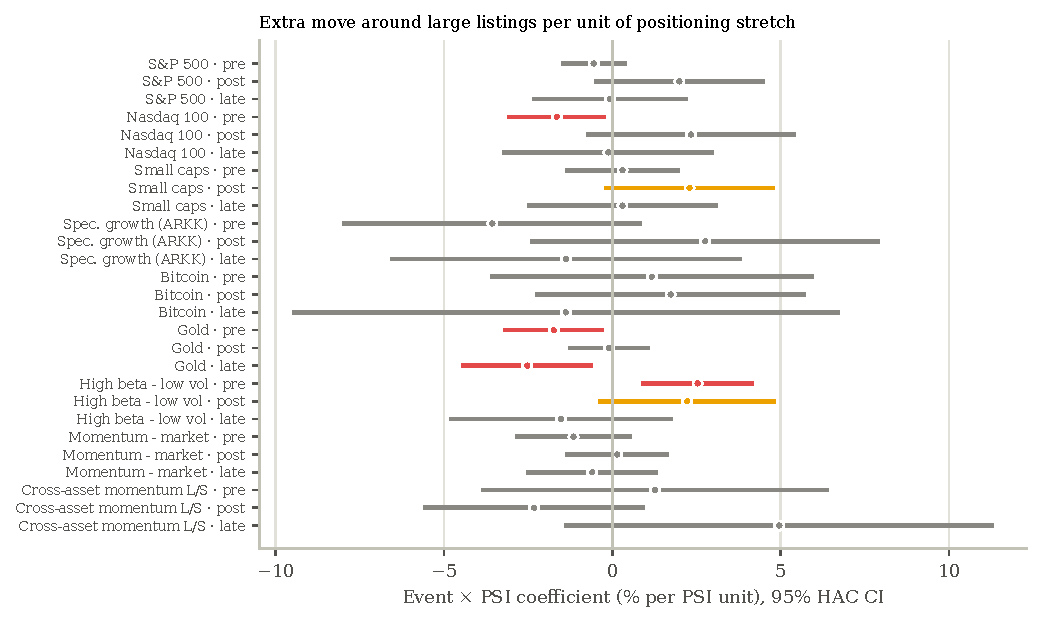
\includegraphics[width=0.9\linewidth]{figures/v2/f4_inter.pdf}
\caption{Event$\times$PSI interaction coefficients with 95\% Newey--West intervals.}\label{fig:inter}
\end{figure}
\begin{table}[!htbp]\centering\footnotesize
\caption{Which state variables line up with the event-window moves?}\label{tab:varcorr}

\begin{threeparttable}
\begin{tabular}{lllrrr}
\toprule
State at T$-$11 & Asset & Window & $\rho$ & $p$ & $q$ \\
\midrule
VIX / VIX3M & Spec. growth (ARKK) & pre & 0.57 & 0.005 & 0.37 \\
CFTC leveraged funds net / OI, E-mini & Bitcoin & pre & 0.56 & 0.007 & 0.37 \\
Bitcoin return, 63d & High beta - low vol & pre & 0.51 & 0.016 & 0.38 \\
CFTC leveraged funds net / OI, E-mini & High beta - low vol & pre & 0.50 & 0.017 & 0.38 \\
CFTC asset managers net / OI, E-mini & High beta - low vol & pre & $-$0.50 & 0.019 & 0.38 \\
Momentum vs market (MTUM/SPY), 63d & Spec. growth (ARKK) & pre & $-$0.44 & 0.038 & 0.57 \\
S\&P 500 return, 63d & Nasdaq 100 & pre & $-$0.44 & 0.042 & 0.57 \\
Momentum vs market (MTUM/SPY), 63d & Bitcoin & pre & $-$0.43 & 0.045 & 0.57 \\
High beta vs low vol (SPHB/SPLV), 63d & Cross-asset momentum L/S & pre & 0.41 & 0.057 & 0.62 \\
VIX / VIX3M & Nasdaq 100 & pre & 0.40 & 0.062 & 0.62 \\
Margin debt growth, YoY (Fed Z.1) & Bitcoin & pre & 0.39 & 0.077 & 0.65 \\
Bitcoin return, 63d & Cross-asset momentum L/S & pre & 0.37 & 0.095 & 0.65 \\
Momentum vs market (MTUM/SPY), 63d & Spec. growth (ARKK) & post & $-$0.36 & 0.098 & 0.65 \\
High beta vs low vol (SPHB/SPLV), 63d & High beta - low vol & pre & 0.36 & 0.099 & 0.65 \\
\bottomrule
\end{tabular}
\begin{tablenotes}[flushleft]\footnotesize
\item \textit{Notes:} Spearman correlation across the 22 large listings between the state variable and the event-window return. The 14 smallest $p$-values of 100 tests are shown; $q$ adjusts across all 100.
\end{tablenotes}
\end{threeparttable}

\end{table}


\subsection{Is liquidity transferred between markets?}
We test three channels directly (Table~\ref{tab:transfer}):
\begin{itemize}
\item \textbf{Peer substitution.} If investors sold listed peers to buy the new issue, the IPO's sector ETF would lag the S\&P~500 around listing. It does not: it is up 0.3\% before listing and 0.4\% through the first week ($p=0.39$ and $0.23$), for all IPOs and for the large ones.
\item \textbf{Attention and volume.} Volume does not rise abnormally in SPY, QQQ, Bitcoin or the sector ETF. It does rise in the recent-IPO complex: the IPO ETF trades abnormally heavily in the listing week ($p=0.003$). Attention moves within the new-issue niche, not across markets.
\item \textbf{Co-selling.} Liquidity-driven selling should raise correlations across assets. On average it does not (SPY--Bitcoin $p=0.95$; SPY--gold correlation falls). The two 2026 episodes are the exception (Table~\ref{tab:correp}; Figure~\ref{fig:transfer}b): SPY and gold moved together with a correlation of 0.88 before SpaceX, and SPY and Bitcoin at 0.74 before Anthropic, against 0.36 on random dates.
\end{itemize}

\begin{table}[!htbp]\centering\footnotesize
\caption{Is liquidity transferred between markets around listings?}\label{tab:transfer}
\resizebox{\linewidth}{!}{
\begin{threeparttable}
\begin{tabular}{lrrrr}
\toprule
Test & $n$ & Events & Random dates & $p$ \\
\midrule
\multicolumn{5}{l}{\textit{Panel A. Peer substitution: own sector ETF minus S\&P~500}} \\
\quad All IPOs, T$-$10 to T$-$1 & 43 & +0.26 & $-$0.22 & 0.39 \\
\quad All IPOs, Listing day to T+5 & 43 & +0.37 & $-$0.14 & 0.23 \\
\quad All IPOs, T+6 to T+20 & 43 & +0.20 & $-$0.45 & 0.37 \\
\quad Large IPOs (\$1bn+), T$-$10 to T$-$1 & 23 & +0.42 & $-$0.21 & 0.41 \\
\quad Large IPOs (\$1bn+), Listing day to T+5 & 23 & +0.08 & $-$0.13 & 0.72 \\
\quad Large IPOs (\$1bn+), T+6 to T+20 & 23 & +0.18 & $-$0.32 & 0.59 \\
\addlinespace
\multicolumn{5}{l}{\textit{Panel B. Abnormal volume around large listings (log ratio to prior 60-day mean)}} \\
\quad S\&P 500 (SPY), T$-$10 to T$-$1 & 23 & $-$0.02 & $-$0.07 & 0.29 \\
\quad S\&P 500 (SPY), Listing week & 23 & $-$0.01 & $-$0.06 & 0.32 \\
\quad Nasdaq (QQQ), T$-$10 to T$-$1 & 23 & +0.02 & $-$0.05 & 0.12 \\
\quad Nasdaq (QQQ), Listing week & 23 & +0.01 & $-$0.05 & 0.29 \\
\quad Recent IPOs (IPO ETF), T$-$10 to T$-$1 & 23 & $-$0.16 & $-$0.25 & 0.43 \\
\quad Recent IPOs (IPO ETF), Listing week & 23 & +0.09 & $-$0.26 & 0.003 \\
\quad Bitcoin, T$-$10 to T$-$1 & 23 & +0.01 & $-$0.05 & 0.30 \\
\quad Bitcoin, Listing week & 23 & $-$0.14 & $-$0.05 & 0.20 \\
\quad Own sector ETF, Listing week & 23 & $-$0.10 & $-$0.09 & 0.93 \\
\addlinespace
\multicolumn{5}{l}{\textit{Panel C. Correlation of daily returns, T$-$10 to T$-$1 (large listings)}} \\
\quad SPY--BTC: level & 23 & +0.26 & +0.36 & 0.16 \\
\quad SPY--BTC: change vs prior 10 sessions & 23 & 0.00 & 0.00 & 0.95 \\
\quad SPY--GLD: level & 23 & +0.07 & +0.19 & 0.19 \\
\quad SPY--GLD: change vs prior 10 sessions & 23 & $-$0.17 & 0.00 & 0.088 \\
\quad BTC--GLD: level & 23 & +0.08 & +0.14 & 0.47 \\
\quad BTC--GLD: change vs prior 10 sessions & 23 & $-$0.11 & 0.00 & 0.25 \\
\quad SPY--IPO ETF: level & 23 & +0.59 & +0.67 & 0.13 \\
\quad SPY--IPO ETF: change vs prior 10 sessions & 23 & +0.02 & 0.00 & 0.75 \\
\bottomrule
\end{tabular}
\begin{tablenotes}[flushleft]\footnotesize
\item \textit{Notes:} Panel A in percent. Random dates: permutation test against 4,000--5,000 random draws (sector drawn in the cohort's proportions for Panel A). Large listings: proceeds of \$1bn or more (23 IPOs).
\end{tablenotes}
\end{threeparttable}
}
\end{table}

\begin{table}[!htbp]\centering\footnotesize
\caption{Cross-asset correlation in the ten sessions before listing}\label{tab:correp}

\begin{threeparttable}
\begin{tabular}{lrrrr}
\toprule
Pair & Random dates & Large listings & SpaceX & Anthropic (to 13 Nov) \\
\midrule
SPY--BTC & +0.36 & +0.26 & +0.30 & +0.74 \\
SPY--GLD & +0.19 & +0.07 & +0.88 & +0.29 \\
BTC--GLD & +0.14 & +0.08 & +0.25 & +0.40 \\
SPY--IPO ETF & +0.67 & +0.59 & +0.89 & +0.89 \\
\bottomrule
\end{tabular}
\begin{tablenotes}[flushleft]\footnotesize
\item \textit{Notes:} Correlation of daily returns over ten sessions. The two 2026 episodes show unusually high co-movement (SPY--gold before SpaceX, SPY--Bitcoin before Anthropic), the signature of a common risk factor rather than of the listings as a group.
\end{tablenotes}
\end{threeparttable}

\end{table}


\subsection{Mechanism: the new stock joins the speculative book}
Why does market crowding at listing predict the fade? One answer is that the new stock is held by the same investors and moves with the same factors as the crowded trades. Regressing each IPO's daily returns on days 2--63 on QQQ, the high-beta spread and Bitcoin gives average betas of 0.85, 0.49 ($t=3.8$) and 0.13 ($t=3.4$) (Table~\ref{tab:betas}; Figure~\ref{fig:transfer}a). New issues are, in effect, levered positions in the speculative complex.

Is the fade then just crowding reversing? No (Table~\ref{tab:reversal}). A stretched high-beta spread does not predict its own reversal over the next 63 days ($t=-0.9$), and after high-PSI listings the spread actually rose. Decomposing each IPO's day 2--63 return, PSI predicts both the factor-implied part ($\rho=-0.34$) and the larger idiosyncratic part ($\rho=-0.41$). Stretched markets mainly lead investors to overpay for the new stock itself, and the overpayment unwinds stock by stock.

\begin{table}[!htbp]\centering\footnotesize
\caption{The IPO joins the speculative book: factor betas over days 2 to 63}\label{tab:betas}

\begin{threeparttable}
\begin{tabular}{lrcrr}
\toprule
Factor & Mean beta & 95\% CI & $t$ & $\rho$ with PSI ($p$) \\
\midrule
QQQ & 0.85 & [0.55, 1.14] & 5.5 & $+$0.01 (0.95) \\
High beta $-$ low vol (SPHB$-$SPLV) & 0.49 & [0.25, 0.75] & 3.8 & $+$0.28 (0.066) \\
Bitcoin & 0.13 & [0.06, 0.21] & 3.4 & -0.05 (0.73) \\
$R^2$ & 0.19 & [0.15, 0.22] & -- & -- \\
\midrule
\multicolumn{5}{l}{\textit{Decomposing the day 2--63 log return; rank correlation with PSI at listing}} \\
\quad Total return & & & & -0.51 ($<$0.001) \\
\quad Factor-implied part & & & & -0.34 (0.027) \\
\quad Idiosyncratic part & & & & -0.41 (0.007) \\
\bottomrule
\end{tabular}
\begin{tablenotes}[flushleft]\footnotesize
\item \textit{Notes:} Each IPO's daily log returns on days 2--63 regressed on QQQ, the high-beta spread and Bitcoin; cross-sectional mean of the 43 betas with bootstrap CI and $t$-statistic. The factor-implied part sums fitted daily returns; the idiosyncratic part sums residuals.
\end{tablenotes}
\end{threeparttable}

\end{table}

\begin{table}[!htbp]\centering\footnotesize
\caption{Does crowding mean-revert after stretched listings?}\label{tab:reversal}
\resizebox{\linewidth}{!}{
\begin{threeparttable}
\begin{tabular}{lrrr}
\toprule
Test & Estimate & $t$ & $p$ \\
\midrule
Slope of next$-$63-day spread return on past-63-day spread return (all days) & -0.13 & -0.9 & 0.35 \\
High-beta spread over the 63 sessions after listing, Low PSI tercile (median) & +10.0\% & -- & -- \\
High-beta spread over the 63 sessions after listing, Mid PSI tercile (median) & $-$0.5\% & -- & -- \\
High-beta spread over the 63 sessions after listing, High PSI tercile (median) & +9.4\% & -- & -- \\
\bottomrule
\end{tabular}
\begin{tablenotes}[flushleft]\footnotesize
\item \textit{Notes:} Newey--West $t$ with 63 lags for the time-series regression (1,554 days). No evidence that crowding unwinds systematically after listings, so the post-IPO fade is not just the factor reversing.
\end{tablenotes}
\end{threeparttable}
}
\end{table}

\begin{figure}[!htbp]\centering
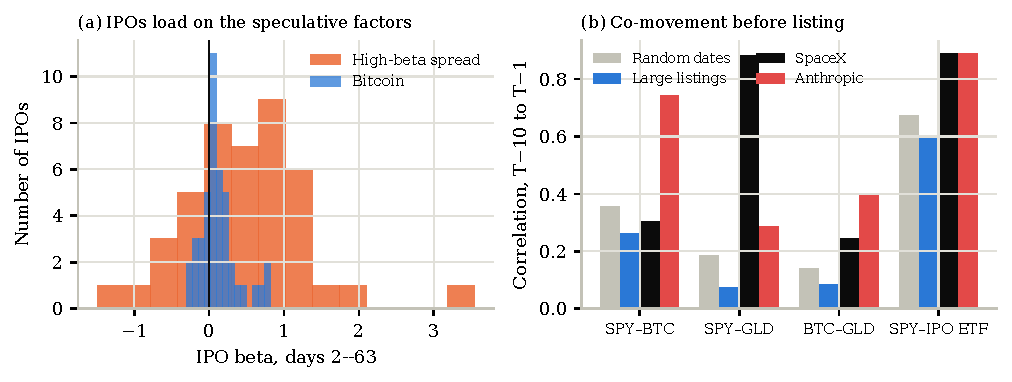
\includegraphics[width=\linewidth]{figures/v3/f_transfer.pdf}
\caption{(a) Distribution of IPO betas to the high-beta spread and to Bitcoin. (b) Cross-asset correlations before listing: random dates, large listings, SpaceX and Anthropic.}\label{fig:transfer}
\end{figure}

% ===========================================================================
\section{What is the relationship? A synthesis}

Table~\ref{tab:lifecycle} assembles the evidence into a lifecycle. The relationship between a large IPO and the rest of the market runs mainly in one direction: from the market's state to the IPO.
\begin{enumerate}
\item \textbf{Bookbuilding sets the pop.} Demand, visible in the price revision, sets how much the stock jumps; crowding into new issues and the IPO's theme adds to it.
\item \textbf{The new stock behaves as a crowded speculative asset.} It loads on the high-beta and crypto factors and attracts attention from the new-issue complex.
\item \textbf{The positioning state at listing sets the fade.} When the market is stretched, investors overpay for the new stock and the excess unwinds over three to six months, mostly idiosyncratically.
\item \textbf{Liquidity transfer is narrow.} We find no broad drain, no peer selling and no average correlation spike. The broad sell-offs around SpaceX and Anthropic coincided with common-factor risk-off episodes (very high correlations, a momentum unwind), which the IPOs may have accompanied but did not, on average, cause.
\end{enumerate}

\begin{table}[!htbp]\centering\footnotesize
\caption{A lifecycle model of a large IPO}\label{tab:lifecycle}
\begin{tabularx}{\linewidth}{@{}p{2.3cm}p{2.1cm}YY@{}}
\toprule
Phase & Window & Main driver & Evidence \\
\midrule
Bookbuilding & Before pricing & Demand; crowding into new issues and the theme & Revision vs pop $\rho=0.67$; IPO-ETF and sector crowding vs pop $\rho\approx0.43$ \\
Opening & Day 1 & Opening auction absorbs the frenzy & Open $+23\%$, close $+19\%$; 60\% close below open; first-hour high in 10/14 \\
Squeeze & Days 2--5 & Momentum, factor exposure & $+5\%$ mean, not significant; betas to high beta and Bitcoin \\
Fade & Days 5--63 & Positioning stretch at listing & PSI vs day 63 $\rho=-0.51$; high-PSI short $+22\%$ \\
Long run & Days 63--252 & Supply, underperformance vs index & Median $-34\%$ vs QQQ at day 126; lock-up window not significant \\
Spillovers & T$-$10 to T+20 & Common risk factor, not the IPO & No average drain; attention to new issues only; high correlation in 2026 episodes \\
\bottomrule
\end{tabularx}
\end{table}

% ===========================================================================
\section{Trading: strategies and implied Sharpe ratios}

Unconditional strategies are weak (Table~\ref{tab:strategies}; Figure~\ref{fig:forest}). Only the allocation flip (offer to first close, $+37\%$, Sharpe 0.72 per trade) is unambiguously profitable, and it requires an allocation. Conditioning helps (Tables~\ref{tab:strat} and~\ref{tab:crowdstrat}). Shorting from day 5 to day 63 earned 2.5\% unconditionally, 13\% when the market was crowded at listing, and 22\% in the top PSI tercile (86\% hit rate, Sharpe 0.81 per trade). The tercile and median splits are in-sample, and borrow costs for new listings are ignored.

\begin{table*}[!htbp]\centering\scriptsize
\caption{Trading strategies on the IPO stock: returns, significance and implied Sharpe ratios}\label{tab:strategies}
\resizebox{\linewidth}{!}{
\begin{threeparttable}
\begin{tabular}{lrrcrrrrrrrl}
\toprule
Strategy & $n$ & Mean & 95\% CI & Median & Hit & $p_t$ & $p_W$ & SR$_\text{trade}$ & SR$_\text{ann}$ & SR$_\text{real}$ & Conf. \\
\midrule
Allocation flip: offer to day-1 close (long) & 43 & +37.1 & [+23, +54] & +19.2 & 79 & $<$0.001 & $<$0.001 & 0.72 & 11.44 & 1.97 & High \\
Buy the open, sell day-1 close (long) & 43 & $-$1.1 & [$-$4, +2] & $-$2.0 & 35 & 0.50 & 0.19 & $-$0.10 & $-$1.63 & $-$0.28 & Low \\
Squeeze: day-1 close to day 5 (long) & 43 & +5.3 & [$-$1, +13] & +4.2 & 58 & 0.16 & 0.54 & 0.22 & 1.71 & 0.59 & Low \\
Fade: short day 5 to day 21 & 43 & +1.7 & [$-$5, +8] & +2.4 & 60 & 0.59 & 0.22 & 0.08 & 0.33 & 0.23 & Low \\
Fade: short day 5 to day 63 & 43 & +2.5 & [$-$12, +15] & +14.3 & 65 & 0.71 & 0.17 & 0.06 & 0.12 & 0.15 & Low \\
Short the open to day 63 & 43 & $-$2.1 & [$-$22, +13] & +10.8 & 56 & 0.82 & 0.39 & $-$0.03 & $-$0.07 & $-$0.09 & Low \\
Lock-up window: short day 118 to day 130 & 42 & $-$0.5 & [$-$5, +4] & +0.5 & 50 & 0.84 & 0.79 & $-$0.03 & $-$0.14 & $-$0.09 & Low \\
Buy day-1 close, hold 1 year (long) & 41 & +0.2 & [$-$19, +20] & $-$15.9 & 44 & 0.99 & 0.90 & 0.00 & 0.00 & 0.01 & Low \\
\midrule
Squeeze vs QQQ: day 1 to 5 & 43 & +4.7 & [$-$2, +12] & +3.7 & 56 & 0.21 & 0.62 & 0.19 & 1.53 & 0.53 & Low \\
Fade vs QQQ: short day 5 to 21 & 43 & +3.4 & [$-$3, +9] & +4.7 & 65 & 0.26 & 0.045 & 0.17 & 0.68 & 0.47 & Medium \\
Fade vs QQQ: short day 5 to 63 & 43 & +8.0 & [$-$6, +20] & +16.9 & 70 & 0.23 & 0.027 & 0.19 & 0.39 & 0.51 & Medium \\
Lock-up vs QQQ: short day 118 to 130 & 42 & $-$1.1 & [$-$6, +4] & $-$1.6 & 45 & 0.69 & 0.61 & $-$0.06 & $-$0.29 & $-$0.17 & Low \\
\bottomrule
\end{tabular}
\begin{tablenotes}[flushleft]\footnotesize
\item \textit{Notes:} Percent per trade; short trades report the short-seller's return. $p_t$: one-sample $t$-test; $p_W$: Wilcoxon signed-rank. SR$_\text{trade}$ = mean/sd per trade; SR$_\text{ann}$ = SR$_\text{trade}\sqrt{252/h}$ for holding period $h$ (an upper bound); SR$_\text{real}$ = SR$_\text{trade}\sqrt{7.5}$, the number of cohort IPOs per year. Confidence: High if the CI excludes zero and $p_W<0.05$; Medium if $\min(p_t,p_W)<0.10$; otherwise Low. Lower block subtracts QQQ.
\end{tablenotes}
\end{threeparttable}
}
\end{table*}

\begin{figure}[!htbp]\centering
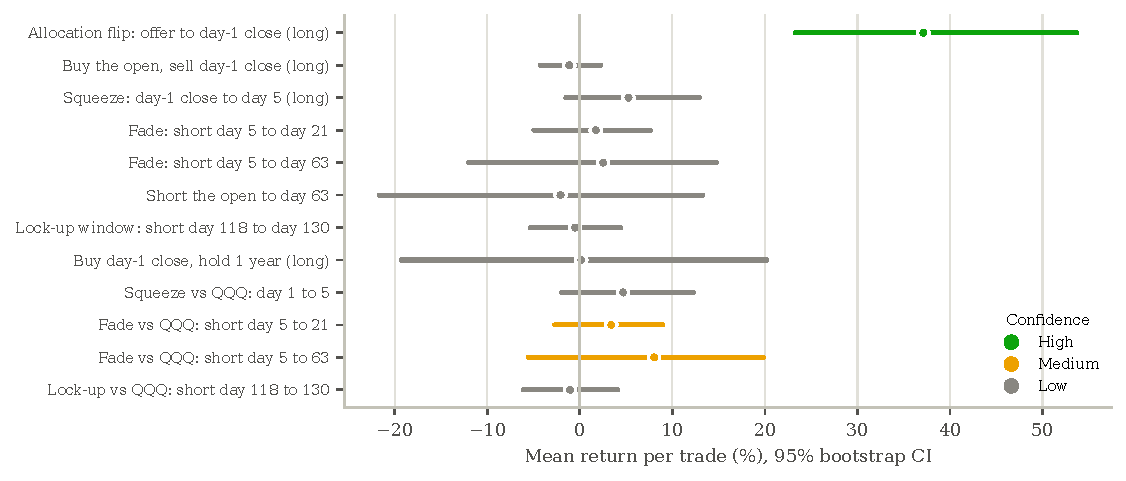
\includegraphics[width=\linewidth]{figures/v1/f5_forest.pdf}
\caption{Mean return per trade with 95\% bootstrap CI, unconditional strategies.}\label{fig:forest}
\end{figure}
\begin{table}[!htbp]\centering\footnotesize
\caption{Positioning-conditioned strategies on the IPO stock}\label{tab:strat}
\resizebox{\linewidth}{!}{
\begin{threeparttable}
\begin{tabular}{lrrcrrrr}
\toprule
Strategy & $n$ & Mean & 95\% CI & Hit & $p_W$ & SR$_\text{trade}$ & SR$_\text{real}$ \\
\midrule
Short day 5 to 63, all IPOs & 43 & +2.5 & [$-$12, +15] & 65 & 0.17 & 0.06 & 0.15 \\
Short day 5 to 63, high-PSI tercile & 14 & +22.4 & [+7, +35] & 86 & 0.013 & 0.81 & 1.26 \\
Short day 5 to 63, low-PSI tercile & 15 & $-$18.8 & [$-$50, +7] & 40 & 0.30 & $-$0.32 & $-$0.51 \\
Long day 1 to 63, low-PSI tercile & 15 & +32.1 & [$-$2, +79] & 53 & 0.19 & 0.38 & 0.61 \\
Short day 5 to 63, high PSI and above range & 12 & +22.2 & [+5, +37] & 83 & 0.034 & 0.74 & 1.06 \\
\bottomrule
\end{tabular}
\begin{tablenotes}[flushleft]\footnotesize
\item \textit{Notes:} Percent per trade; shorts report the short-seller's return. SR$_\text{real}$ scales the per-trade Sharpe by the square root of the number of qualifying IPOs per year in the cohort (5.75 years). The tercile split uses the full-sample PSI distribution, so these are in-sample results; costs and borrow are ignored.
\end{tablenotes}
\end{threeparttable}
}
\end{table}

\begin{table}[!htbp]\centering\footnotesize
\caption{Short from day 5 to day 63, conditioned on crowding}\label{tab:crowdstrat}

\begin{threeparttable}
\begin{tabular}{lrrcrrr}
\toprule
Subset & $n$ & Mean & 95\% CI & Hit & $p_W$ & SR$_\text{trade}$ \\
\midrule
All & 43 & +2.5 & [$-$12, +15] & 65 & 0.17 & 0.06 \\
Crowded & 22 & +13.3 & [$-$1, +26] & 77 & 0.039 & 0.41 \\
Not crowded & 21 & $-$8.8 & [$-$33, +11] & 52 & 0.79 & $-$0.17 \\
Crowded and above range & 17 & +10.0 & [$-$7, +25] & 71 & 0.21 & 0.28 \\
High day-1 turnover & 22 & $-$2.2 & [$-$27, +17] & 64 & 0.39 & $-$0.04 \\
\bottomrule
\end{tabular}
\begin{tablenotes}[flushleft]\footnotesize
\item \textit{Notes:} Short-seller's return in percent. In-sample split at the cohort median; costs and borrow ignored.
\end{tablenotes}
\end{threeparttable}

\end{table}


% ===========================================================================
\section{Hypotheses: tested and open}

Table~\ref{tab:hyptested} lists the 14 hypotheses tested in this paper with their verdicts. Table~\ref{tab:hypopen} sets out 12 further hypotheses, each with a test design and the data it needs; several become testable once Anthropic has traded.

\begin{table}[!htbp]\centering\scriptsize
\caption{Hypotheses tested in this paper}\label{tab:hyptested}
\begin{tabularx}{\linewidth}{@{}p{0.5cm}p{3.6cm}YYp{1.6cm}@{}}
\toprule
\# & Hypothesis & Prediction & Result & Verdict \\
\midrule
H1 & Mega-IPO cash call drains other risk assets & Risk assets fall T$-$10 to T$-$1 & Bitcoin $+3.6\%$ ($p=0.67$); no asset significant ($q>0.3$) & Rejected \\
H2 & Drain occurs only in stretched markets & Event$\times$PSI $<0$ before listing & Only surviving interaction is positive (high beta, $q=0.05$) & Not supported \\
H3 & Investors sell listed peers & Sector ETF lags S\&P around listing & $+0.3\%$ / $+0.4\%$, $p\geq0.23$ & Rejected \\
H4 & Attention moves to new issues & Abnormal volume in new-issue complex & IPO ETF volume up in listing week, $p=0.003$; none in SPY, QQQ, BTC, sector & Supported (narrow) \\
H5 & Liquidity-driven co-selling & Correlations rise before listings & No average rise; high in SpaceX (SPY--gold 0.88) and Anthropic (SPY--BTC 0.74) & Episode-specific \\
H6 & Partial adjustment & Price revision predicts pop & $\rho=0.67$, $q<0.001$ & Supported \\
H7 & Hot deals revert & Above-range deals fade more & Day 63 $-20\%$ (CI $-28$ to $-2$); day 126 $q=0.52$ & Partly supported \\
H8 & Positioning sets the fade & PSI predicts day-63 return & $\rho=-0.51$, $q=0.006$; robust to demand, 2021 & Supported \\
H9 & Crowded trades drive it within buckets & Crowding predicts fade inside buckets & Within-bucket permutation $p=0.010$--$0.028$ in 6 of 8 bucketings & Supported \\
H10 & The IPO joins the speculative book & Betas to high-beta and crypto factors & 0.49 ($t=3.8$), 0.13 ($t=3.4$) & Supported \\
H11 & The fade is crowding reversing & Factor reversal after stretched listings & No reversal ($t=-0.9$); idiosyncratic part dominates & Rejected \\
H12 & Flipping predicts the fade & Day-1 turnover predicts returns & All $p>0.35$ & Rejected \\
H13 & The opening print is the high & Close below open; early high & 60\% below open; first-hour high in 10/14 & Supported (descriptive) \\
H14 & Size, sector, season and rates matter & Bucket medians differ & Kruskal--Wallis $q\geq0.57$ & Not supported \\
\bottomrule
\end{tabularx}
\end{table}

\begin{table}[!htbp]\centering\scriptsize
\caption{Open hypotheses for further work}\label{tab:hypopen}
\begin{tabularx}{\linewidth}{@{}p{0.5cm}p{3.4cm}YY@{}}
\toprule
\# & Hypothesis & Test design & Data needed \\
\midrule
A1 & Retail allocation and retail flow amplify pop and fade & Pop and fade against retail share of the book and retail net buying & Allocation by investor type; retail broker flow \\
A2 & Option listing triggers a gamma squeeze around days 3--5 & Returns around the first options day against call volume and dealer gamma & OPRA volumes, open interest by strike \\
A3 & Index fast entry is front-run, then sold on the news & Abnormal returns before and after inclusion dates; demand vs passive ownership & Inclusion announcements, passive AUM (SpaceX fell about 13\% after Nasdaq-100 entry) \\
A4 & Staggered, earnings-linked unlocks create supply shocks & Abnormal returns and volume in each unlock window & S-1 lock-up schedules; unlock calendars \\
A5 & The fade starts when borrow becomes available & Returns after borrow fee and utilisation changes & Securities-lending data, short interest \\
A6 & Pre-IPO secondary prices predict the pop & Pop against the secondary-market premium to the offer & Forge or EquityZen prices; prediction markets \\
A7 & Funding stress turns IPO weeks into co-selling & Interact events with SOFR--IORB, repo spreads, prime-broker leverage & FRED funding spreads; OFR prime-broker data \\
A8 & Holders are revalued at pricing & Abnormal returns of strategic holders (Alphabet, Amazon for Anthropic) around pricing & Stake sizes from filings; intraday prices on 18--19 Nov \\
A9 & Volatility targeting transmits IPO-week volatility & Exposure changes of vol-control strategies after vol spikes & Model-implied vol-target exposure \\
A10 & Crypto is a funding leg for allocations & Exchange inflows and stablecoin redemptions around mega-listings & On-chain flow data \\
A11 & A listing re-rates its theme & Comparable stocks against the pricing surprise (price vs range) & Comparable set (AI infrastructure, model developers) \\
A12 & Supply crowding weakens pops & Pop against IPO proceeds raised in the previous 60 days & Full IPO calendar with proceeds \\
\bottomrule
\end{tabularx}
\end{table}

% ===========================================================================
\section{Application: SpaceX and Anthropic}

\paragraph{SpaceX listed into a stretched market.} Eleven sessions before its June listing, SpaceX met realised volatility at the 21st percentile and a steep volatility curve (VIX/VIX3M at the 14th). High beta was at the 92nd percentile, momentum crowding at the 98th and asset managers' E-mini length at the 92nd; PSI was at the 90th percentile and crowding at the 86th percentile of the cohort (Table~\ref{tab:case}; Figure~\ref{fig:dash}). FINRA margin debt peaked at \$1.50tn at the end of June and fell 5.6\% in July (Figure~\ref{fig:unwind}). The stock popped 19\%, peaked on day 3 and was below its offer by day 23, as the high-PSI tercile predicts.

\paragraph{Anthropic lists after an unwind.} At the public S-1 on 26 October the market was calm but not stretched (PSI 45th percentile). Since then crowded trades have unwound (Table~\ref{tab:moves}). High beta lost 4.6\% against low volatility and momentum 2.3\% against the market; Bitcoin fell 12.5\% and MSTR 19.5\%. SPY--Bitcoin correlation reached 0.74. By 13 November, momentum crowding was at its lowest reading since 2020, PSI at the 12th percentile and the crowding composite below that of any of the 43 listings in the cohort. Overall leverage remains high: margin-debt growth is at the 83rd percentile and asset managers' E-mini length at the 82nd.

\begin{table}[!htbp]\centering\footnotesize
\caption{SpaceX and Anthropic: the state of positioning}\label{tab:case}
\resizebox{\linewidth}{!}{
\begin{threeparttable}
\begin{tabular}{lrrrr}
\toprule
Variable & SpaceX, T$-$11 & ANT, S-1 public & ANT, T$-$11 & ANT, 13 Nov \\
\midrule
S\&P 500 realised vol, 21d & 10.2 (21) & 10.0 (18) & 11.3 (31) & 21.7 (85) \\
S\&P 500 return, 63d & +9.5 (80) & +3.3 (37) & $-$2.0 (18) & $-$2.4 (17) \\
VIX / VIX3M & 0.82 (14) & 0.92 (72) & 0.98 (92) & 0.94 (77) \\
High beta vs low vol (SPHB/SPLV), 63d & +24.2 (92) & +2.2 (47) & $-$8.7 (10) & $-$15.4 (2) \\
Momentum vs market (MTUM/SPY), 63d & +12.6 (98) & $-$2.5 (33) & $-$8.4 (6) & $-$13.6 (0) \\
Bitcoin return, 63d & +9.0 (51) & +25.3 (68) & +19.7 (61) & +5.8 (47) \\
CFTC leveraged funds net / OI, E-mini & $-$0.19 (19) & $-$0.19 (20) & $-$0.20 (14) & $-$0.19 (23) \\
CFTC asset managers net / OI, E-mini & 0.49 (92) & 0.47 (81) & 0.47 (85) & 0.47 (82) \\
Margin debt growth, YoY (Fed Z.1) & +30.5 (75) & +46.6 (83) & +46.6 (83) & +46.6 (83) \\
Positioning stretch index (PSI) & 0.80 (90) & 0.02 (45) & $-$0.56 (20) & $-$0.90 (12) \\
\bottomrule
\end{tabular}
\begin{tablenotes}[flushleft]\footnotesize
\item \textit{Notes:} Value (percentile rank since June 2020). SpaceX T$-$11 = 27 May 2026; Anthropic S-1 public = 26 October 2026; Anthropic T$-$11 = 3 November 2026.
\end{tablenotes}
\end{threeparttable}
}
\end{table}

\begin{table}[!htbp]\centering\footnotesize
\caption{The sell-offs: SpaceX pre-listing window and Anthropic so far}\label{tab:moves}

\begin{threeparttable}
\begin{tabular}{lrr}
\toprule
Asset & SpaceX, T$-$10 to T$-$1 & Anthropic, 3--13 Nov \\
\midrule
Bitcoin & $-$14.6 & $-$12.5 \\
MSTR & $-$23.3 & $-$19.5 \\
ARKK & $-$7.1 & $-$6.9 \\
Semis (SMH) & +1.6 & $-$6.3 \\
Nasdaq 100 & $-$2.5 & $-$0.8 \\
Gold & $-$6.6 & $-$1.1 \\
High beta $-$ low vol & $-$2.2 & $-$4.6 \\
Momentum $-$ market & +3.6 & $-$2.3 \\
\bottomrule
\end{tabular}
\begin{tablenotes}[flushleft]\footnotesize
\item \textit{Notes:} Log returns in percent. Anthropic's window covers 8 of its 10 pre-listing sessions.
\end{tablenotes}
\end{threeparttable}

\end{table}

\begin{figure}[!htbp]\centering
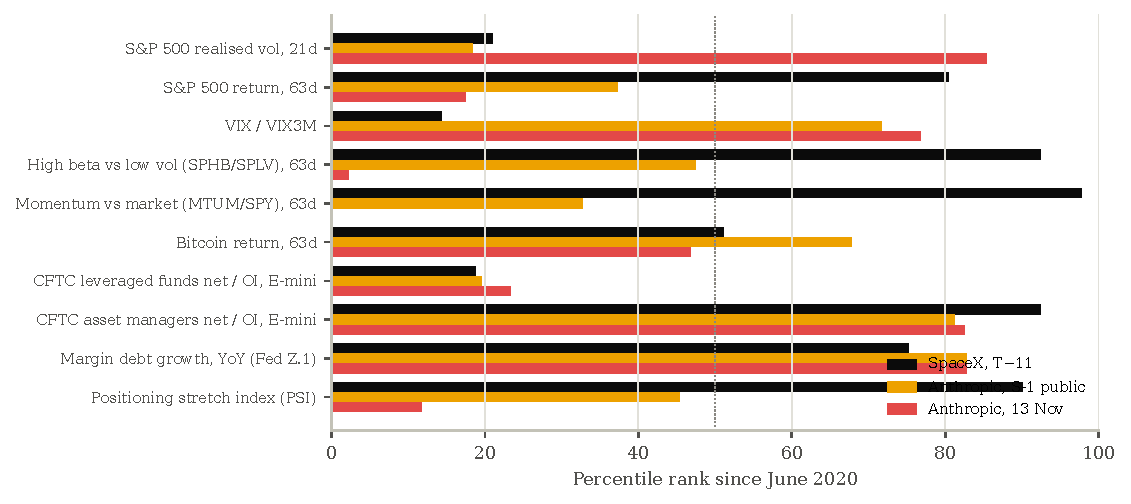
\includegraphics[width=0.9\linewidth]{figures/v2/f2_dashboard.pdf}
\caption{Percentile rank of each state variable: SpaceX at T$-$11, Anthropic at its public S-1 and on 13 November.}\label{fig:dash}
\end{figure}
\begin{figure}[!htbp]\centering
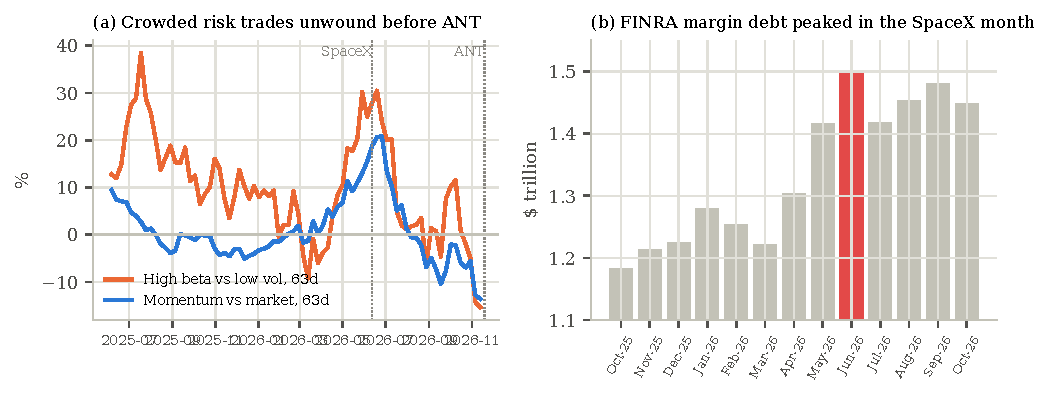
\includegraphics[width=\linewidth]{figures/v2/f5_unwind.pdf}
\caption{(a) High beta vs low volatility and momentum vs the market, 63-day relative returns. (b) FINRA margin debt.}\label{fig:unwind}
\end{figure}

\paragraph{Outlook.} Anthropic is a de-risked listing in a still-levered market. The cohort's low-PSI, low-crowding listings popped less and did not fade on average. Demand remains the main driver of the pop: pricing above the \$70--78 range would point to a large first day. Positioning points to a shallower fade than SpaceX's, unless crowding rebuilds quickly into and after the listing. Two risks lie outside the IPO itself: Anthropic is far larger than any low-PSI listing in the sample, and the remaining leverage could unwind further. Table~\ref{tab:tree} gives the conditional outlook by pricing and Table~\ref{tab:cal} the calendar.

\begin{table*}[!htbp]\centering\footnotesize
\caption{Conditional outlook by Anthropic's pricing}\label{tab:tree}

\begin{threeparttable}
\begin{tabular}{lrrrrrp{5.2cm}}
\toprule
Anthropic prices\ldots & $n$ & Pop & D21 & D63 & D126 & Historical edge (no allocation) \\
\midrule
Above \$78 (above range) & 28 & +32 & $-$2 & $-$20 & $-$27 & Fade day 5$\to$63: +11.5\%, hit 71\%, $p_W=0.028$ \\
\$70--78 or below & 14 & +4 & +1 & +14 & +7 & No reliable fade \\
\bottomrule
\end{tabular}
\begin{tablenotes}[flushleft]\footnotesize
\item \textit{Notes:} Cohort medians in percent for the two demand groups. Anthropic's range is \$70--78 for 825 million shares.
\end{tablenotes}
\end{threeparttable}

\end{table*}

\begin{table}[!htbp]\centering\small
\caption{Anthropic event calendar}\label{tab:cal}

\begin{threeparttable}
\begin{tabular}{llr}
\toprule
Event & Trading day & Date \\
\midrule
Pricing (after the close) & T$-$1 & Wed 18 Nov 2026 \\
Day 1: first trade & Day 1 & Thu 19 Nov 2026 \\
Day 5 & Day 5 & Wed 25 Nov 2026 \\
Day 13: SpaceX lock-up expiry & Day 13 & Tue 08 Dec 2026 \\
Day 21 & Day 21 & Fri 18 Dec 2026 \\
Day 63 & Day 63 & Mon 22 Feb 2027 \\
Day 126 (about 180 days) & Day 126 & Fri 21 May 2027 \\
\bottomrule
\end{tabular}
\begin{tablenotes}[flushleft]\footnotesize
\item \textit{Notes:} Day 1 = first close (19 November 2026). NYSE holidays applied (Thanksgiving, Christmas, New Year, MLK, Presidents' Day, Good Friday). SpaceX's 8 December lock-up expiry is Anthropic's day 13.
\end{tablenotes}
\end{threeparttable}

\end{table}

\begin{table}[!htbp]\centering\footnotesize
\caption{How unusual is the run-up to Anthropic?}\label{tab:runup}

\begin{threeparttable}
\begin{tabular}{lrrr}
\toprule
Asset & 14-session move & Percentile & $z$ \\
\midrule
S\&P 500 (SPY) & $$-$$1.4 & 22 & $-$0.67 \\
Nasdaq 100 (QQQ) & $$-$$4.5 & 13 & $-$1.16 \\
Small caps (IWM) & $+$0.2 & 44 & $-$0.12 \\
Speculative growth (ARKK) & $$-$$8.4 & 18 & $-$0.91 \\
Semis (SMH) & $$-$$10.1 & 6 & $-$1.59 \\
Software (IGV) & $$-$$9.2 & 6 & $-$1.59 \\
Bitcoin & $$-$$14.7 & 8 & $-$1.16 \\
Gold (GLD) & $$-$$3.4 & 14 & $-$1.01 \\
Long Treasuries (TLT) & $$-$$2.4 & 26 & $-$0.64 \\
Dollar (UUP) & $+$1.7 & 82 & $+$0.95 \\
High yield (HYG) & $+$0.2 & 45 & $-$0.04 \\
VIX (points) & $+$0.9 & 64 & $+$0.21 \\
US 10Y (bp) & $+$16.8 & 75 & $+$0.64 \\
Recent IPOs (IPO ETF) & $$-$$3.6 & 27 & $-$0.53 \\
\bottomrule
\end{tabular}
\begin{tablenotes}[flushleft]\footnotesize
\item \textit{Notes:} Move over the 14 sessions to 13 November 2026, ranked against every 14-session window since mid-2020.
\end{tablenotes}
\end{threeparttable}

\end{table}


% ===========================================================================
\section{Limitations}
\begin{itemize}
\item \textbf{Samples.} 43 IPOs and 22 large listings, hand-selected and clustered in hot windows; effective sample sizes are smaller than the counts.
\item \textbf{Measurement.} PSI and the crowding composite are equal-weighted and standardised on the full sample. CFTC leveraged-fund positions mix direction with basis trades. Z.1 margin data are quarterly. FINRA data cover only 13 months. Prime-brokerage, options and retail-flow data were not available.
\item \textbf{In-sample strategies.} Splits use full-sample breakpoints; borrow costs and options timing are ignored.
\item \textbf{Confounding.} Eleven to 22 events cannot separate IPO effects from contemporaneous macro news.
\item \textbf{Anthropic terms.} The range, share count and lock-up come from secondary summaries of the S-1/A and should be verified against the filing.
\end{itemize}

\section{Conclusion}
A newly listed stock follows a recognisable path: demand sets its pop, the opening print is usually the day's high, and the market's positioning at listing sets how far it fades. The stock trades as part of the speculative book, so crowded trades around it, not frenzied trading in it, carry the signal, and that signal holds across size, season, rate, volatility, float and demand buckets. Large listings do not systematically pull liquidity from other markets; attention moves to new issues, while broad sell-offs around mega-listings coincide with common-factor risk-off episodes. SpaceX listed at the top of the positioning cycle and behaved accordingly. Anthropic lists after the crowded trades have unwound, which points to a smaller pop and a shallower fade, while leverage in the wider market remains a risk of its own.

\vspace{1em}
\noindent{\footnotesize\textit{Disclaimer.} This paper is for research and discussion. It is not investment advice or a recommendation to buy or sell any security. Figures for Anthropic are based on public filings and press reports as of 15 November 2026.}

\bibliographystyle{plainnat}
\bibliography{refs}

\clearpage
\appendix
\section{Appendix}
\begin{table}[!htbp]\centering\small
\caption{Large-listing events used in the cross-asset study}\label{tab:events}

\begin{threeparttable}
\begin{tabular}{llr}
\toprule
Listing date & Company & Proceeds (\$bn) \\
\midrule
2020-09-16 & Snowflake & 3.4 \\
2020-12-09 & DoorDash + Airbnb & 6.9 \\
2021-03-11 & Coupang & 4.6 \\
2021-07-29 & Robinhood & 2.1 \\
2021-11-10 & Rivian & 11.9 \\
2023-09-14 & Arm & 4.9 \\
2024-07-25 & Lineage & 4.4 \\
2025-03-28 & CoreWeave & 1.5 \\
2025-12-17 & Medline & 6.3 \\
2026-06-12 & SpaceX & 75 \\
2026-07-10 & SK hynix ADR & 26.5 \\
\bottomrule
\end{tabular}
\begin{tablenotes}[flushleft]\footnotesize
\item \textit{Notes:} DoorDash and Airbnb listed one day apart and are treated as one event. SK hynix is a cross-listing of an already-public company.
\end{tablenotes}
\end{threeparttable}

\end{table}

\begin{table*}[!htbp]\centering\scriptsize
\caption{Market state before each large listing (percentile ranks)}\label{tab:states}
\resizebox{\linewidth}{!}{
\begin{threeparttable}
\begin{tabular}{llrrrrrrrrrrr}
\toprule
Listed & Company & \$bn & RV21 & Mom63 & VIX/3M & $\beta$ spread & MTUM & BTC & Lev.\ funds & Margin & PSI & PSI pct \\
\midrule
2020-09-16 & Snowflake + Unity & 4.66 & 5 & 94 & 17 & 44 & 90 & 64 & 53 & 23 & 0.63 & 83 \\
2020-12-09 & DoorDash + Airbnb & 6.86 & 88 & 41 & 56 & 90 & 37 & 89 & 88 & 56 & 0.24 & 62 \\
2021-01-13 & Affirm & 1.21 & 9 & 89 & 39 & 95 & 41 & 97 & 88 & 56 & 1.46 & 98 \\
2021-02-11 & Bumble & 2.15 & 59 & 85 & 98 & 93 & 54 & 96 & 79 & 79 & 0.57 & 80 \\
2021-03-03 & Oscar Health & 1.42 & 65 & 88 & 1 & 97 & 89 & 99 & 76 & 79 & 1.79 & 100 \\
2021-03-11 & Coupang & 4.55 & 64 & 85 & 15 & 97 & 57 & 98 & 69 & 79 & 1.48 & 98 \\
2021-07-29 & Robinhood & 2.09 & 17 & 60 & 3 & 27 & 13 & 1 & 83 & 96 & 0.11 & 52 \\
2021-11-10 & Rivian & 11.93 & 53 & 42 & 4 & 61 & 83 & 84 & 92 & 88 & 0.50 & 76 \\
2023-09-14 & Arm & 4.87 & 44 & 65 & 45 & 57 & 59 & 41 & 44 & 8 & 0.14 & 54 \\
2023-10-11 & Birkenstock & 1.48 & 41 & 17 & 86 & 25 & 53 & 24 & 43 & 8 & $-$0.60 & 19 \\
2024-05-01 & Viking & 1.54 & 36 & 59 & 91 & 50 & 91 & 82 & 36 & 48 & $-$0.01 & 43 \\
2024-07-25 & Lineage & 4.44 & 0 & 73 & 53 & 36 & 53 & 21 & 52 & 52 & 0.16 & 56 \\
2024-10-02 & StandardAero & 1.44 & 54 & 35 & 47 & 14 & 28 & 32 & 67 & 52 & $-$0.26 & 29 \\
2025-01-24 & Venture Global & 1.75 & 62 & 40 & 74 & 55 & 48 & 86 & 39 & 44 & 0.02 & 45 \\
2025-02-13 & SailPoint & 1.38 & 59 & 42 & 67 & 47 & 63 & 86 & 21 & 60 & 0.06 & 48 \\
2025-03-28 & CoreWeave & 1.5 & 72 & 4 & 98 & 2 & 64 & 21 & 58 & 60 & $-$1.37 & 4 \\
2025-06-05 & Circle & 1.05 & 65 & 15 & 46 & 14 & 81 & 53 & 52 & 31 & $-$0.41 & 24 \\
2025-07-31 & Figma & 1.22 & 10 & 97 & 33 & 98 & 81 & 78 & 27 & 40 & 1.25 & 96 \\
2025-09-10 & Klarna + Figure + Gemini & 2.58 & 36 & 87 & 13 & 87 & 28 & 44 & 25 & 40 & 0.68 & 85 \\
2025-12-17 & Medline & 6.27 & 59 & 58 & 21 & 76 & 28 & 19 & 25 & 64 & 0.20 & 58 \\
2026-06-12 & SpaceX & 75 & 21 & 80 & 14 & 92 & 98 & 51 & 19 & 75 & 0.80 & 90 \\
2026-07-10 & SK hynix ADR & 26.5 & 69 & 92 & 68 & 92 & 99 & 25 & 16 & 75 & 0.29 & 65 \\
\midrule
-- & Anthropic, T-11 (3 Nov 2026) & -- & 31 & 18 & 92 & 10 & 6 & 61 & 14 & 83 & $-$0.56 & 20 \\
-- & Latest (13 Nov 2026) & -- & 85 & 17 & 77 & 2 & 0 & 47 & 23 & 83 & $-$0.90 & 12 \\
-- & Anthropic S-1 public (26 Oct 2026) & -- & 18 & 37 & 72 & 47 & 33 & 68 & 20 & 83 & 0.02 & 45 \\
\bottomrule
\end{tabular}
\begin{tablenotes}[flushleft]\footnotesize
\item \textit{Notes:} Percentile ranks (0--100) of each state variable against all days June 2020 to November 2026, measured at T$-$11 (the close before the pre-listing window). Low RV21 and low VIX/VIX3M are the stretched readings for those columns. Anthropic's T$-$11 is 3 November 2026; its S-1 became public on 26 October.
\end{tablenotes}
\end{threeparttable}
}
\end{table*}

\begin{table}[!htbp]\centering\footnotesize
\caption{Strategies on the subsets closest to Anthropic}\label{tab:subsets}

\begin{threeparttable}
\begin{tabular}{lrcrrrl}
\toprule
Subset / trade & Mean & 95\% CI & Hit & $p_W$ & SR$_\text{trade}$ & Conf. \\
\midrule
\multicolumn{7}{l}{\textit{Large and mega caps (\$30B+)} ($n=10$)} \\
\quad Squeeze: day 1 to 5 & +12.2 & [$-$9, +39] & 40 & 0.92 & 0.30 & Low \\
\quad Fade: short day 5 to 21 & +10.4 & [+1, +20] & 60 & 0.28 & 0.62 & Medium \\
\quad Fade: short day 5 to 63 & +9.1 & [$-$14, +32] & 70 & 0.43 & 0.24 & Low \\
\multicolumn{7}{l}{\textit{Software, AI \& semis} ($n=12$)} \\
\quad Squeeze: day 1 to 5 & +3.2 & [$-$7, +14] & 58 & 0.73 & 0.16 & Low \\
\quad Fade: short day 5 to 21 & +7.5 & [+2, +14] & 75 & 0.052 & 0.68 & Medium \\
\quad Fade: short day 5 to 63 & $-$18.8 & [$-$58, +12] & 50 & 0.62 & $-$0.28 & Low \\
\multicolumn{7}{l}{\textit{Listed with 10Y rising} ($n=15$)} \\
\quad Squeeze: day 1 to 5 & $-$1.0 & [$-$8, +6] & 40 & 0.42 & $-$0.07 & Low \\
\quad Fade: short day 5 to 21 & +2.4 & [$-$6, +11] & 53 & 0.64 & 0.13 & Low \\
\quad Fade: short day 5 to 63 & +12.3 & [+1, +24] & 73 & 0.11 & 0.52 & Medium \\
\multicolumn{7}{l}{\textit{Day-1 pop 15-40\% (SpaceX-like)} ($n=12$)} \\
\quad Squeeze: day 1 to 5 & +8.7 & [$-$2, +22] & 75 & 0.20 & 0.37 & Low \\
\quad Fade: short day 5 to 21 & +3.4 & [$-$6, +12] & 75 & 0.42 & 0.21 & Low \\
\quad Fade: short day 5 to 63 & $-$3.9 & [$-$24, +16] & 42 & 0.79 & $-$0.11 & Low \\
\multicolumn{7}{l}{\textit{Priced above initial range} ($n=28$)} \\
\quad Squeeze: day 1 to 5 & +4.1 & [$-$3, +12] & 57 & 0.69 & 0.20 & Low \\
\quad Fade: short day 5 to 21 & $-$0.4 & [$-$9, +7] & 64 & 0.33 & $-$0.02 & Low \\
\quad Fade: short day 5 to 63 & +11.5 & [0, +22] & 71 & 0.028 & 0.37 & Medium \\
\multicolumn{7}{l}{\textit{Float under 8\% (ANT ~4.5\%)} ($n=13$)} \\
\quad Squeeze: day 1 to 5 & +4.0 & [$-$11, +24] & 38 & 0.79 & 0.11 & Low \\
\quad Fade: short day 5 to 21 & +7.3 & [$-$4, +18] & 62 & 0.22 & 0.35 & Low \\
\quad Fade: short day 5 to 63 & $-$9.8 & [$-$52, +23] & 69 & 1.00 & $-$0.14 & Low \\
\bottomrule
\end{tabular}
\begin{tablenotes}[flushleft]\footnotesize
\item \textit{Notes:} As Table~\ref{tab:strategies}. Anthropic is a large, low-float software/AI listing pricing into a rising-yield market; whether it prices above range is known only on 18 November.
\end{tablenotes}
\end{threeparttable}

\end{table}

\begin{table}[!htbp]\centering\scriptsize
\caption{Cross-asset trades around large listings}\label{tab:xtrades}

\begin{threeparttable}
\begin{tabular}{llrrrrrr}
\toprule
Asset & Trade & Mean & vs typical & Hit & $p$ & SR$_\text{event}$ & SR$_\text{real}$ \\
\midrule
Bitcoin & Short T-10 to T-1 & $-$3.6 & $-$1.5 & 45 & 0.67 & $-$0.33 & $-$0.44 \\
Bitcoin & Long T+1 to T+5 & +0.4 & $-$0.6 & 55 & 0.79 & 0.07 & 0.09 \\
Bitcoin & Long T+6 to T+20 & +10.5 & +7.4 & 82 & 0.11 & 0.37 & 0.49 \\
Speculative growth (ARKK) & Short T-10 to T-1 & $-$0.7 & $-$0.1 & 45 & 0.97 & $-$0.10 & $-$0.13 \\
Speculative growth (ARKK) & Long T+1 to T+5 & $-$2.8 & $-$3.0 & 45 & 0.095 & $-$0.46 & $-$0.61 \\
Speculative growth (ARKK) & Long T+6 to T+20 & +4.2 & +3.5 & 73 & 0.27 & 0.38 & 0.50 \\
Gold (GLD) & Short T-10 to T-1 & +0.1 & +0.7 & 45 & 0.51 & 0.02 & 0.03 \\
Gold (GLD) & Long T+1 to T+5 & $-$0.1 & $-$0.4 & 55 & 0.63 & $-$0.03 & $-$0.04 \\
Gold (GLD) & Long T+6 to T+20 & +1.1 & +0.3 & 55 & 0.83 & 0.24 & 0.32 \\
Nasdaq 100 (QQQ) & Short T-10 to T-1 & +0.5 & +1.4 & 55 & 0.26 & 0.12 & 0.16 \\
Nasdaq 100 (QQQ) & Long T+1 to T+5 & $-$1.1 & $-$1.5 & 55 & 0.087 & $-$0.27 & $-$0.36 \\
Nasdaq 100 (QQQ) & Long T+6 to T+20 & +3.8 & +2.6 & 73 & 0.083 & 0.81 & 1.07 \\
Semis (SMH) & Short T-10 to T-1 & +1.1 & +2.7 & 73 & 0.17 & 0.14 & 0.19 \\
Semis (SMH) & Long T+1 to T+5 & $-$1.2 & $-$2.0 & 45 & 0.16 & $-$0.17 & $-$0.23 \\
Semis (SMH) & Long T+6 to T+20 & +5.9 & +3.7 & 82 & 0.11 & 0.79 & 1.05 \\
Software (IGV) & Short T-10 to T-1 & $-$0.3 & +0.3 & 36 & 0.86 & $-$0.06 & $-$0.08 \\
Software (IGV) & Long T+1 to T+5 & $-$1.2 & $-$1.5 & 45 & 0.21 & $-$0.28 & $-$0.38 \\
Software (IGV) & Long T+6 to T+20 & +4.2 & +3.4 & 82 & 0.077 & 0.52 & 0.70 \\
Recent IPOs (IPO ETF) & Short T-10 to T-1 & $-$1.3 & $-$0.8 & 36 & 0.69 & $-$0.23 & $-$0.31 \\
Recent IPOs (IPO ETF) & Long T+1 to T+5 & $-$1.6 & $-$1.8 & 55 & 0.22 & $-$0.27 & $-$0.36 \\
Recent IPOs (IPO ETF) & Long T+6 to T+20 & +2.7 & +2.2 & 82 & 0.36 & 0.33 & 0.45 \\
\bottomrule
\end{tabular}
\begin{tablenotes}[flushleft]\footnotesize
\item \textit{Notes:} Percent per event, 11 events. ``vs typical'' subtracts the average of all same-length windows. SR$_\text{real}$ scales by $\sqrt{1.8}$ listings per year.
\end{tablenotes}
\end{threeparttable}

\end{table}

\begin{scriptsize}\setlength{\tabcolsep}{2.6pt}
\begin{longtable}{llllrrrrlrrr}
\caption{The IPO cohort}\label{tab:cohort}\\
\toprule
Company & Ticker & Listed & Sector & Offer & Cap \$bn & Proceeds \$m & Float \% & vs range & Pop & D21 & D63 \\
\midrule
\endfirsthead
\toprule Company & Ticker & Listed & Sector & Offer & Cap \$bn & Proceeds \$m & Float \% & vs range & Pop & D21 & D63 \\ \midrule
\endhead
\bottomrule \multicolumn{12}{l}{\scriptsize Returns in percent; D21/D63 from the day-1 close. Sources: SEC 424B4, company pricing releases, Yahoo Finance.} \\ \endlastfoot
Snowflake & SNOW & 2020-09-16 & Software & 120 & 33.3 & 3,360 & 10.1 & Above & +112 & $-$4 & +30 \\
Unity & U & 2020-09-18 & Software & 52 & 20.3 & 1,300 & 6.4 & Above & +31 & +35 & +115 \\
DoorDash & DASH & 2020-12-09 & Consumer internet & 102 & 38.3 & 3,366 & 8.8 & Above & +86 & $-$18 & $-$24 \\
Airbnb & ABNB & 2020-12-10 & Consumer internet & 68 & 47.3 & 3,490 & 7.4 & Above & +113 & +2 & +43 \\
Affirm & AFRM & 2021-01-13 & Fintech & 49 & 12.5 & 1,205 & 9.6 & Above & +97 & +45 & $-$29 \\
Bumble & BMBL & 2021-02-11 & Consumer internet & 43 & 8.2 & 2,150 & 26.2 & Above & +64 & $-$1 & $-$33 \\
Oscar Health & OSCR & 2021-03-03 & Fintech & 39 & 7.6 & 1,419 & 18.7 & Above & $-$11 & $-$23 & $-$27 \\
Coupang & CPNG & 2021-03-11 & Consumer internet & 35 & 64.2 & 4,550 & 7.1 & Above & +41 & $-$7 & $-$23 \\
Compass & COMP & 2021-04-01 & Consumer internet & 18 & 3.0 & 450 & 15.0 & Below & +12 & $-$6 & $-$35 \\
Duolingo & DUOL & 2021-07-28 & Software & 102 & 4.0 & 521 & 13.0 & Above & +32 & $-$5 & +40 \\
Robinhood & HOOD & 2021-07-29 & Fintech & 38 & 32.0 & 2,090 & 6.5 & Within & $-$8 & +35 & +14 \\
Toast & TOST & 2021-09-22 & Software & 40 & 20.0 & 870 & 4.3 & Above & +56 & $-$18 & $-$45 \\
Rivian & RIVN & 2021-11-10 & Industrials & 78 & 66.0 & 11,934 & 18.1 & Above & +29 & +15 & $-$36 \\
Nextracker & NXT & 2023-02-09 & Industrials & 24 & 3.5 & 638 & 18.2 & Above & +27 & +2 & +9 \\
Cava & CAVA & 2023-06-15 & Consumer & 22 & 2.5 & 318 & 13.0 & Above & +99 & +9 & $-$18 \\
Arm & ARM & 2023-09-14 & Software & 51 & 54.5 & 4,870 & 8.9 & Within & +25 & $-$18 & +2 \\
Instacart & CART & 2023-09-19 & Consumer internet & 30 & 10.0 & 660 & 6.6 & Above & +12 & $-$27 & $-$27 \\
Klaviyo & KVYO & 2023-09-20 & Software & 30 & 9.2 & 576 & 6.3 & Above & +9 & $-$6 & $-$14 \\
Birkenstock & BIRK & 2023-10-11 & Consumer & 46 & 8.1 & 1,484 & 18.2 & Within & $-$13 & +5 & +19 \\
Astera Labs & ALAB & 2024-03-20 & Software & 36 & 5.4 & 713 & 13.2 & Above & +72 & +14 & +8 \\
Reddit & RDDT & 2024-03-21 & Consumer internet & 34 & 4.9 & 748 & 15.3 & Within & +48 & $-$19 & +14 \\
Ibotta & IBTA & 2024-04-19 & Consumer & 88 & 2.7 & 577 & 21.7 & Above & +11 & +8 & $-$34 \\
Rubrik & RBRK & 2024-04-25 & Software & 32 & 5.6 & 752 & 13.4 & Above & +16 & $-$11 & $-$7 \\
Viking & VIK & 2024-05-01 & Consumer & 24 & 10.4 & 1,537 & 14.8 & Within & +9 & +17 & +37 \\
Waystar & WAY & 2024-06-07 & Healthcare & 21.5 & 3.7 & 968 & 26.1 & Within & $-$4 & 0 & +32 \\
Tempus AI & TEM & 2024-06-14 & Healthcare & 37 & 6.2 & 411 & 6.7 & Within & +9 & +1 & +23 \\
Lineage & LINE & 2024-07-25 & Industrials & 78 & 19.6 & 4,437 & 22.6 & Above & +4 & +5 & $-$2 \\
StandardAero & SARO & 2024-10-02 & Industrials & 24 & 8.0 & 1,440 & 17.9 & Above & +36 & $-$10 & $-$24 \\
Venture Global & VG & 2025-01-24 & Industrials & 25 & 60.5 & 1,750 & 2.9 & Below & $-$4 & $-$37 & $-$64 \\
SailPoint & SAIL & 2025-02-13 & Software & 23 & 12.8 & 1,380 & 10.8 & Within & $-$4 & $-$15 & $-$14 \\
CoreWeave & CRWV & 2025-03-28 & Software & 40 & 23.0 & 1,500 & 6.5 & Below & 0 & +5 & +300 \\
eToro & ETOR & 2025-05-13 & Fintech & 52 & 4.2 & 620 & 14.8 & Above & 0 & +21 & $-$2 \\
Hinge Health & HNGE & 2025-05-22 & Healthcare & 32 & 2.6 & 437 & 16.8 & Within & +17 & +16 & +49 \\
Circle & CRCL & 2025-06-05 & Fintech & 31 & 6.8 & 1,054 & 15.5 & Above & +168 & +149 & +41 \\
Chime & CHYM & 2025-06-12 & Fintech & 27 & 11.6 & 864 & 7.4 & Above & +37 & $-$19 & $-$35 \\
Figma & FIG & 2025-07-31 & Software & 33 & 19.3 & 1,219 & 6.3 & Above & +250 & $-$38 & $-$55 \\
Figure & FIGR & 2025-09-11 & Fintech & 25 & 5.3 & 788 & 14.9 & Above & +24 & +54 & +30 \\
Klarna & KLAR & 2025-09-11 & Fintech & 40 & 15.1 & 1,372 & 9.1 & Above & +7 & $-$3 & $-$28 \\
Gemini & GEMI & 2025-09-12 & Fintech & 28 & 3.3 & 425 & 12.8 & Above & +14 & $-$27 & $-$65 \\
StubHub & STUB & 2025-09-17 & Consumer internet & 23.5 & 8.6 & 800 & 9.3 & Within & $-$6 & $-$12 & $-$36 \\
Netskope & NTSK & 2025-09-18 & Software & 19 & 7.3 & 908 & 12.4 & Above & +18 & +1 & $-$11 \\
Medline & MDLN & 2025-12-17 & Healthcare & 29 & 40.0 & 6,265 & 15.7 & Within & +41 & +8 & +6 \\
SpaceX & SPCX & 2026-06-12 & Industrials & 135 & 1,770.0 & 75,000 & 4.2 & -- & +19 & $-$15 & $-$6 \\
\end{longtable}
\end{scriptsize}


\end{document}
